\documentclass[11pt]{article}
\usepackage{amsmath,amssymb,amsthm}

\newtheorem{proposition}{Proposition}
\newtheorem{corollary}{Corollary}
\newtheorem{remark}{Remark}
\usepackage{amsthm}
\usepackage[sort]{natbib}
\usepackage{pifont}
\usepackage{array}
\usepackage{bbding}
\usepackage{booktabs}
\usepackage[flushleft]{threeparttable}
\usepackage{textcomp}
\usepackage{graphicx}
\usepackage{url}
\usepackage{makeidx}
\usepackage{multirow}
\usepackage{multicol}
%\renewcommand{\familydefault}{\rmdefault}
\usepackage[T1]{fontenc}
%\usepackage[latin9]{inputenc}
\usepackage[a4paper]{geometry}
\geometry{verbose,tmargin=20mm,bmargin=20mm,lmargin=35mm,rmargin=20mm,footskip=0.5cm}
\pagestyle{plain}
\usepackage[usenames,dvipsnames]{xcolor}
\definecolor{dukeblue}{rgb}{0.0, 0.0, 0.61}
\definecolor{phthaloblue}{rgb}{0.0, 0.06, 0.54}
\usepackage{setspace}
\usepackage[english]{babel}
\setlength{\emergencystretch}{2em}
\usepackage{commath}
\usepackage{dsfont}
%\usepackage[sfmath]{kpfonts} %% sfmath option only to make math in sans serif. Probably only for use when the base font is sans serif.
%\renewcommand*\familydefault{\sfdefault} %% Only if the base font of the document is to be sans serif
%\usepackage[bitstream-charter]{mathdesign}
\usepackage[T1]{fontenc}
\normalfont
%     \usepackage{mathpazo}
%
\usepackage{libertine}



\title{Is ``the Empty Planet''  unavoidable: \\
Does Long-run Economic Growth Must Lead to Population Decline?}%}%\thanks{The author thanks  the Monash Macroeconomics discussion group  for valuable comments on the paper.}}
\author{Ratbek Dzhumashev\thanks{Department of Economics, Monash University, Wellington Rd., Clayton VIC 3800, Australia and Centre for Applied Macroeconomic Analysis, Australian National University, Australia.           e-mail: \texttt{Ratbek.Dzhumashev@monash.edu}} 	
}

\date{}
\begin{document}
\maketitle
\begin{abstract}
\noindent
\citet{jones22} shows how population decline can undermine idea production and lead to stagnant living standards. \citet{STRULIK2024104943} demonstrates that human-capital accumulation can sustain economic growth despite a shrinking workforce. His analysis focuses on population decline; although his bounded idea-growth specification also permits growth at replacement fertility, it does not provide a habitat-based mechanism that draws fertility towards replacement.

This paper introduces such a mechanism. Preferences for children increase with habitat per capita, while habitat declines with aggregate economic activity. The household solution remains in closed form, with contemporaneous fertility determined through a within-period general-equilibrium condition. With fixed habitat, a unique replacement-fertility equilibrium exists under a crossing condition and is locally stable when the demographic response is sufficiently moderate. With endogenous habitat, a positive limiting habitat floor is required for a positive stationary population alongside unbounded output. The iso-elastic specification admits a positive balanced-growth path under population decline, but that path is unstable; convergence towards replacement fertility therefore requires a separate analysis of transitional growth and does not imply stagnation. Following Strulik, we adopt bounded logistic idea growth to obtain a finite limiting growth rate. Conditional on population converging to a positive stationary level, $(1+\sigma)\theta>1$ implies that effective research input per unit of knowledge diverges and idea growth converges to its ceiling. A ceiling calibrated to the benchmark delivers approximately 1.84 percent annual per-capita income growth. Under these convergence and saturation conditions, a fixed remediation tax affects levels and transitions but leaves the limiting growth rate unchanged.

\end{abstract}

\section{Introduction}
\citet{jones22} examines the unintended economic consequences of a declining global population. In standard idea-based growth models, sustained progress depends on a constant—or rising—pool of researchers. As fertility in many high-income economies falls below replacement, Jones highlights the risk of an “Empty Planet” outcome: as population dwindles, idea production slows and living standards ultimately stagnate. Although a social planner could, in principle, avert this scenario through timely fertility policy, Jones argues that implementation delays can push the economy into a self-reinforcing trap of negative growth. In this view, the long-run fate of economic progress depends on whether societies can prevent sustained demographic decline. The choice between an “Expanding Cosmos” of rising prosperity and terminal stagnation may therefore turn on contemporary fertility trends.

Jones's pessimism follows from treating raw labour as the key input into idea creation. \citet{STRULIK2024104943}, by contrast, emphasises human capital embodied in an educated workforce. Aggregate human capital can continue to expand even as the number of workers falls, allowing sustained growth despite population decline. His iso-elastic specification admits a positive balanced-growth path under suitable parameter restrictions, but that path is not asymptotically stable. He therefore introduces a bounded logistic idea-growth law under which the economy can converge to a finite positive growth rate.

We build on this distinction between balanced-growth existence and dynamic convergence. Strulik's logistic condition also permits sustained growth at replacement fertility; our contribution is to introduce habitat feedback that can make replacement fertility an endogenous demographic outcome. The iso-elastic balanced-growth formula cannot establish what happens along a trajectory on which fertility approaches replacement. We therefore use the bounded specification to study finite limiting growth conditional on demographic stabilisation, rather than infer stagnation from the iso-elastic formula.

A recurring objection to bounded idea-growth laws is that their positive lower bound appears to
permit ``innovation without people''. We show below that this objection does not bear on the
equilibrium of interest. When the habitat feedback stabilises population at a strictly positive
level, the relevant limit is the \emph{upper} bound: provided $(1+\sigma)\theta>1$ --- a condition
comfortably satisfied by the calibration --- human capital grows fast enough relative to the
knowledge stock that effective research input per unit of knowledge diverges, and idea growth
saturates at its ceiling $\bar g_A$. Sustained growth alongside a stable population is therefore
driven by a research input that keeps expanding in efficiency units, not by ideas arriving without
researchers.



\citet{dao25} highlight that the time cost of raising children increases at a diminishing rate with population density. Higher
population density reduces the space available for raising children, drives up housing costs, and consequently demands more time
from women for childcare. This assumption helps generate population stabilization in the long run.
This connection has been pioneered by \citet{goodsell} and \citet{thompson}, and was used by \citet{DELACROIX2012271} and
\citet{DAO2013442} to explain fertility rates being negatively affected by population density. More recently,
\citet{DELACROIX201713} provide empirical evidence confirming this idea. According to \citet{DELACROIX2012271}, controlling
pollution either through Pigovian taxes or tradable quotas encourages agents to shift away from production to tax-free activities
such as procreation and leisure. This can gradually impoverish successive generations: population tends to increase and production
per capita tends to decrease as generations pass.
Therefore, the above models can be further extended by assuming that  fertility preference are habitat-dependent. We present such an extension of Jones-Strulik model in the next section.


Specifically, we allow fertility to be influenced not only by income constraints but also by the limits imposed by the human habitat. This second channel operates through the availability of biological resources, which depends on environmental quality. Environmental degradation then affects effective fertility by lowering child survival rates. In this respect, we extend \citet{mari10} and \citet{Varvarigos2013} by adding biological resource constraints to the environmental effects on fertility that arise through health.


A second strand of research examines how production and consumption affect environmental quality. The relationship between economic activity and environmental degradation has been modelled in two contrasting ways. One view, represented by \citet{raffin14}, \citet{econ2008}, and \citet{marsiglio2018}, argues that output growth can improve environmental quality when abatement efforts are sufficiently strong to offset pollution emissions. In contrast, \citet{Varvarigos2013} and \citet{pautrel08} contend that production growth inevitably degrades environmental quality despite abatement activities. Extending this debate, \citet{mar2017} show that environmental quality depends on both aggregate output and population size, with the latter contributing through consumption-based emissions. Because environmental quality affects health, mortality, and fertility decisions, these studies highlight an important link between economic growth and long-run demographic outcomes, underscoring the need to coordinate environmental and demographic policies.

Dzhumashev  and Kazakevitch (2025) show that the amount of resources used in production directly increases pollution and causes environmental deterioration. Income growth and a fall in the quality of the environment raise the relative cost of living and affect fertility negatively. This leads to a trade-off between income growth and population growth. Despite these insights, the literature has not fully considered material resource use as a fundamental source of environmental degradation or examined how the resulting deterioration of environmental and biological conditions shapes the long-run interaction between economic growth and population dynamics. While \citet{Varvarigos2013}, \citet{pautrel08}, and \citet{mar2017} analyze the effects of pollution on environmental quality, health, and fertility, they largely abstract from material resource extraction as the underlying driver of environmental pressure. Moreover, little attention has been paid to how the depletion of biological resources may reinforce the demographic consequences of sustained economic expansion. Although the present paper does not model these channels separately, it captures their combined effects through the impact of production on environmental quality. Incorporating this mechanism into the Jones-Strulik framework allows us to examine whether sustained economic growth necessarily leads to population decline or can instead coexist with a stable long-run demographic equilibrium.




%%==========================================================
\section{Habitat-Dependent Fertility Taste (Habitat per Capita and Closed-Form Household Solution)}
\label{sec:habitat_taste}
%%==========================================================
\subsection{Time, demography, and habitat per capita}
Time is discrete, $t=0,1,2,\dots$. In each period, a generation of homogeneous adults makes fertility and education decisions for
their children, who become workers in period $t+1$. There is no physical capital.

Let $L_t$ denote the adult population (workforce size), $n_t$ fertility (children per adult), $h_t$ human capital per worker, and
$\ell_t$ labor supply per worker (time devoted to work). Aggregate human capital used in production is
\begin{align}
H_t &= h_t \,\ell_t\, L_t. \label{eq:Hagg_hab}
\end{align}
Population evolves according to
\begin{align}
L_{t+1} &= n_t L_t. \label{eq:Llaw_hab}
\end{align}

Let $E_t$ denote the (exogenous for now but to be relaxed in next section) size of the human habitat and define habitat per capita
\begin{align}
\epsilon_t \equiv \frac{E_t}{L_t}. \label{eq:eps_def}
\end{align}
The key modification is that the taste for children depends positively on habitat per capita:
\begin{align}
\alpha_t \equiv \alpha(\epsilon_t),
\qquad
\alpha'(\epsilon)>0. \label{eq:alpha_eps}
\end{align}
In a large economy, an individual household takes $\epsilon_t$ (hence $\alpha_t$) as given at time $t$.

\subsection{Production and ideas}
Final output is produced with aggregate human capital $H_t$ and a stock of ideas $A_t$:
\begin{align}
Y_t &= A_t^{\sigma} H_t, \qquad \sigma \ge 0. \label{eq:Y_hab}
\end{align}
Ideas evolve through learning-by-doing:
\begin{align}
A_{t+1}-A_t &= A_t^{1-\beta} H_t^{\lambda},
\qquad \beta \ge 0,\ \lambda \ge 0. \label{eq:Aiso_hab}
\end{align}
Competitive factor markets imply the wage per unit of human capital is
\begin{align}
w_t &= \frac{\partial Y_t}{\partial H_t}=A_t^{\sigma}. \label{eq:wage_hab}
\end{align}

\subsection{Households: preferences, constraints, and human-capital formation}
Adults value consumption $c_t$, children $n_t$, and the human capital of their children $h_{t+1}$:
\begin{align}
u_t &= \log c_t + \alpha(\epsilon_t)\log n_t + \gamma \log h_{t+1},
\qquad \gamma>0. \label{eq:util_hab}
\end{align}
Raising one child costs $\phi$ units of adult time. Parents also spend $s_t$ units of time per child on education (teacher time),
and $q_t$ units of goods per child on education. Hence labor supply is
\begin{align}
\ell_t &= 1-\phi n_t - s_t n_t. \label{eq:labor_hab}
\end{align}
The budget constraint is
\begin{align}
w_t h_t (1-\phi n_t - s_t n_t) &= c_t + q_t n_t. \label{eq:budget_hab}
\end{align}
Human capital of the next generation is produced with diminishing returns in both education inputs:
\begin{align}
h_{t+1} &= \nu\, q_t^{\theta} s_t^{\eta},
\qquad \nu>0,\ 0<\theta<1,\ 0<\eta<1. \label{eq:hc_hab}
\end{align}

Using \eqref{eq:hc_hab}, period utility can be written as
\begin{align}
u_t
&=\log c_t + \alpha(\epsilon_t)\log n_t + \gamma\theta \log q_t + \gamma\eta \log s_t + \text{const}.
\label{eq:util_hab_reduced}
\end{align}
For brevity define
\begin{align}
\Gamma \equiv \gamma(\eta+\theta). \label{eq:Gamma_def_hab}
\end{align}

\subsection{Household problem and closed-form solution}
The household chooses $(c_t,n_t,s_t,q_t)$ to maximize \eqref{eq:util_hab_reduced} subject to
\eqref{eq:budget_hab}--\eqref{eq:hc_hab}. Because $\alpha(\epsilon_t)$ is taken as a time-$t$ parameter, the optimal policy rules
have the same closed form as in the baseline model by Strulik (2024), with $\alpha$ replaced by $\alpha(\epsilon_t)$.

\begin{proposition}[Optimal choices with $\alpha=\alpha(\epsilon_t)$ and $\alpha'(\epsilon)>0$]
\label{prop:hab_solution}
Assume an interior solution with $\alpha(\epsilon_t)>\Gamma$. Then the household's optimal choices are
\begin{align}
c_t
&=\frac{w_t h_t}{1+\alpha(\epsilon_t)},
\label{eq:sol_c_hab}\\[4pt]
n_t
&= n(\epsilon_t)
\equiv
\frac{\alpha(\epsilon_t)-\Gamma}{\phi\left(1+\alpha(\epsilon_t)\right)},
\label{eq:sol_n_hab}\\[4pt]
s_t
&= s(\epsilon_t)
\equiv
\frac{\eta\gamma\phi}{\alpha(\epsilon_t)-\Gamma},
\label{eq:sol_s_hab}\\[4pt]
q_t
&= q(\epsilon_t)\, w_t h_t,
\qquad
q(\epsilon_t)\equiv
\frac{\gamma\theta\phi}{\alpha(\epsilon_t)-\Gamma},
\label{eq:sol_q_hab}\\[4pt]
\ell_t
&=1-\phi n_t - s_t n_t
=\frac{1+\gamma\theta}{1+\alpha(\epsilon_t)}.
\label{eq:sol_l_hab}
\end{align}
\end{proposition}

\subsection{Comparative statics with respect to habitat per capita}
Since $n(\epsilon)$ is increasing in $\alpha$ and $\alpha'(\epsilon)>0$, fertility is increasing in habitat per capita:
\begin{align}
\frac{\partial n(\epsilon)}{\partial \epsilon}
&=
\underbrace{\frac{\partial n}{\partial \alpha}}_{=\ \frac{1+\Gamma}{\phi(1+\alpha)^2}>0}
\alpha'(\epsilon)
>0.
\label{eq:dn_deps_pos_hab}
\end{align}
Per-child education inputs decrease with $\epsilon$ (because they fall with $\alpha$):
\begin{align}
\frac{\partial s(\epsilon)}{\partial \epsilon}
&=
\underbrace{\frac{\partial s}{\partial \alpha}}_{=\ -\frac{\eta\gamma\phi}{(\alpha-\Gamma)^2}<0}
\alpha'(\epsilon)
<0,
\label{eq:ds_deps_neg_hab}
\\
\frac{\partial q(\epsilon)}{\partial \epsilon}
&=
\underbrace{\frac{\partial q}{\partial \alpha}}_{=\ -\frac{\gamma\theta\phi}{(\alpha-\Gamma)^2}<0}
\alpha'(\epsilon)
<0.
\label{eq:dq_deps_neg_hab}
\end{align}
Consumption and labor supply also decrease with $\epsilon$:
\begin{align}
\frac{\partial c_t}{\partial \epsilon_t}
&=
-\frac{w_t h_t}{(1+\alpha(\epsilon_t))^2}\alpha'(\epsilon_t)<0,
\label{eq:dc_deps_neg_hab}\\
\frac{\partial \ell_t}{\partial \epsilon_t}
&=
-\frac{1+\gamma\theta}{(1+\alpha(\epsilon_t))^2}\alpha'(\epsilon_t)<0.
\label{eq:dl_deps_neg_hab}
\end{align}

\subsection{Aggregate dynamics implied by the habitat-dependent solution}
Given the policy rules, aggregate human capital is
\begin{align}
H_t = h_t\,\ell(\epsilon_t)\,L_t,
\qquad
\ell(\epsilon_t)\equiv \frac{1+\gamma\theta}{1+\alpha(\epsilon_t)}.
\label{eq:Hlaw_hab}
\end{align}
Using $w_t=A_t^{\sigma}$ from \eqref{eq:wage_hab} in \eqref{eq:sol_q_hab}--\eqref{eq:hc_hab}, human capital evolves as
\begin{align}
h_{t+1}
&= \nu\,\big(q(\epsilon_t)\, w_t h_t\big)^{\theta}\, s(\epsilon_t)^{\eta}
= \nu\,q(\epsilon_t)^{\theta}s(\epsilon_t)^{\eta}\,A_t^{\sigma\theta}\,h_t^{\theta}.
\label{eq:h_law_hab}
\end{align}
Population evolves as
\begin{align}
L_{t+1}=n(\epsilon_t)L_t.
\label{eq:Llaw_mod_hab}
\end{align}
Ideas evolve according to
\begin{align}
A_{t+1}-A_t
&= A_t^{1-\beta}\,\Big(h_t\,\ell(\epsilon_t)\,L_t\Big)^{\lambda}.
\label{eq:A_law_hab}
\end{align}

\subsection{Induced habitat-per-capita dynamics}
From $\epsilon_t=E_t/L_t$ and \eqref{eq:Llaw_mod_hab},
\begin{align}
\epsilon_{t+1}
=\frac{E_{t+1}}{L_{t+1}}
=
\frac{E_{t+1}}{E_t}\cdot \frac{\epsilon_t}{n(\epsilon_t)}.
\label{eq:eps_law_general_hab}
\end{align}
If habitat is fixed ($E_{t+1}=E_t$), then
\begin{align}
\epsilon_{t+1}
= f(\epsilon_t)
\equiv
\frac{\epsilon_t}{n(\epsilon_t)}.
\label{eq:eps_law_fixedE_hab}
\end{align}

\begin{remark}[Stationary $\epsilon$ and local stability when $E$ is fixed]
\label{rem:eps_stability_hab}
A stationary $\epsilon^\ast$ satisfies $\epsilon^\ast=f(\epsilon^\ast)$, i.e.
\[
n(\epsilon^\ast)=1 \text{ and } \eqref{eq:sol_n_hab}
\quad\Longleftrightarrow\quad
\alpha(\epsilon^\ast)=\frac{\phi+\Gamma}{1-\phi}
\qquad (\phi<1).
\]
If $\alpha(\cdot)$ is strictly increasing, this pins down a unique $\epsilon^\ast$.

Local stability of $\epsilon^\ast$ under \eqref{eq:eps_law_fixedE_hab} requires $|f'(\epsilon^\ast)|<1$.
Since
\[
f'(\epsilon)=\frac{n(\epsilon)-\epsilon n'(\epsilon)}{n(\epsilon)^2},
\]
at $n(\epsilon^\ast)=1$ we obtain
\[
f'(\epsilon^\ast)=1-\epsilon^\ast n'(\epsilon^\ast).
\]
Hence a necessary and sufficient condition for local stability is
\[
0<\epsilon^\ast n'(\epsilon^\ast)<2.
\]
Under $\alpha'(\epsilon)>0$ we have $n'(\epsilon)>0$ and thus $f'(\epsilon^\ast)<1$:
the habitat--fertility link induces a negative feedback that can stabilize $\epsilon_t$ when habitat is fixed.
\end{remark}

\section{Calibration and comparison: $\alpha(\epsilon)$ vs.\ constant $\alpha$}
\label{sec:calibration}

\subsection{Parameter values (from Strulik, 2024)}
We adopt the calibrated preference/education parameters
\[
\alpha_0=0.39,\quad \gamma=0.26,\quad \eta=0.07,\quad \phi=0.138,\quad \theta=0.83,
\]
and the ideas/goods technology parameters
\[
\sigma=1,\quad \lambda=\tfrac{3}{4},\quad \beta=2.
\]
Define $\Gamma\equiv \gamma(\eta+\theta)$ and assume a generation lasts $G=30$ years
(annual growth rate: $(1+g)^{1/G}-1$).

\subsection{Closed-form allocations as functions of $\alpha_t$}
For any given $\alpha_t>\Gamma$ (interior solution), the household rules are
\[
n(\alpha)=\frac{\alpha-\Gamma}{\phi(1+\alpha)},\qquad
s(\alpha)=\frac{\eta\gamma\phi}{\alpha-\Gamma},\qquad
q_t=\underbrace{\frac{\gamma\theta\phi}{\alpha-\Gamma}}_{\equiv q^{\ast}(\alpha)}\,w_t h_t,
\]
and labor supply per worker is
\[
\ell(\alpha)=\frac{1+\gamma\theta}{1+\alpha}.
\]

\subsection{Balanced-growth mapping from fertility}
On a balanced-growth path (BGP) with constant $n$ and strictly positive constant idea growth, the basic model implies
\[
1+g_h=\left(\frac{1}{n}\right)^{\frac{\lambda\sigma\theta}{\lambda\sigma\theta-\beta(1-\theta)}},\qquad
(1+g_A)^\beta=\big((1+g_h)n\big)^\lambda,
\]
and per-capita income grows as
\[
1+g_y=(1+g_A)^{\sigma}(1+g_h),
\qquad y_t=A_t^\sigma\,h_t\,\ell.
\]

\subsection{Case A: constant $\alpha=\alpha_0$}
With $\alpha=\alpha_0$ constant,
\[
n_0=n(\alpha_0),\quad s_0=s(\alpha_0),\quad q^{\ast}_0=q^{\ast}(\alpha_0),\quad \ell_0=\ell(\alpha_0),
\]
and the BGP growth rates follow from the mapping above.

\subsection{Case B: habitat feedback $\alpha(\epsilon)$ with $\alpha'(\epsilon)>0$}
Let habitat per capita be $\epsilon_t\equiv E/L_t$ and assume
\[
\alpha_t=\alpha(\epsilon_t),\qquad \alpha'(\epsilon)>0.
\]
For calibration we use the power form (normalized at $\epsilon=1$):
\[
\alpha(\epsilon)=\alpha_0\,\epsilon^{\xi},\qquad \alpha(\,1\,)=\alpha_0.
\]
Assume fixed habitat $E_{t+1}=E_t\equiv E$ and normalize $(E,L_0)=(1,1)$ so $\epsilon_0=1$.

\paragraph{Pinning down $\xi$ (illustrative target).}
In this model, replacement fertility $n=1$ occurs at the unique preference level
\[
\alpha^\star \ \text{s.t.}\ n(\alpha^\star)=1
\quad\Longrightarrow\quad
\alpha^\star=\frac{\phi+\Gamma}{1-\phi}.
\]
We choose $\xi$ so that when habitat per capita doubles ($\epsilon=2$, i.e.\ population halves under fixed $E$),
the taste for children reaches replacement:
\[
\alpha(2)=\alpha^\star
\quad\Longrightarrow\quad
\xi=\frac{\ln(\alpha^\star/\alpha_0)}{\ln 2}.
\]
Then the induced law of motion is
\[
L_{t+1}=n\!\big(\alpha(E/L_t)\big)\,L_t,
\]
which converges to a fixed point with $n=1$ (here: $L^\star=0.5$, $\epsilon^\star=2$ by construction).

\paragraph{Growth implication: balanced-growth existence and dynamic convergence.}
The iso-elastic specification admits a positive balanced-growth path under population decline when
$\lambda\sigma\theta>\beta(1-\theta)$, but this path is not asymptotically stable
\citep[Sections~2.4--2.5]{STRULIK2024104943}. The growth-rate mapping above describes a family
of such paths indexed by constant fertility. Its limit as $n\uparrow1$ is not the time limit of
growth along a trajectory on which $n_t\to1$.

At replacement fertility, constant positive growth would require both
$(1+g_A)^\beta=(1+g_h)^\lambda$ and
$(1+g_h)^{1-\theta}=(1+g_A)^{\sigma\theta}$, hence
\[
\big[\beta(1-\theta)-\lambda\sigma\theta\big]\ln(1+g_A)=0.
\]
Unless $\lambda\sigma\theta=\beta(1-\theta)$, no finite strictly positive constant-growth BGP
exists at $n=1$. This does not establish stagnation. The original accumulation equation continues
to generate ideas at positive states, and the economy need not approach a constant-growth path.
Indeed, under the present calibration, zero limiting idea growth is inconsistent with convergence
to a positive stationary population.\footnote{Suppose $L_t\to L^\ast>0$,
$\alpha_t\to\alpha^\ast>\Gamma$ and $g_{A,t}\to0$. Write
$h_{t+1}=C_t A_t^{\sigma\theta}h_t^\theta$, with $C_t\to C>0$, and set
$p=\sigma\theta/(1-\theta)$ and $v_t=\ln h_t-p\ln A_t$. Then
$v_{t+1}=\theta v_t+\ln C_t-p\ln(1+g_{A,t})$, so
$h_t/A_t^p\to C^{1/(1-\theta)}>0$. The stock $A_t$ must diverge: a finite positive limit
would imply positive limiting human capital and hence a positive limiting increment to $A_t$.
It follows that $g_{A,t}\sim K A_t^{\lambda p-\beta}$ for some $K>0$.
Here $\lambda p-\beta=1.6618>0$, contradicting $g_{A,t}\to0$.}
Endogenous convergence towards replacement therefore requires a separate analysis of transitional
growth. Following Strulik, we adopt bounded logistic idea growth to obtain a finite limiting
growth rate alongside demographic stabilisation.

\subsection{Numerical results}
Compute $\Gamma=\gamma(\eta+\theta)=0.234$ and
\[
\alpha^\star=\frac{\phi+\Gamma}{1-\phi}=0.431555,\qquad
\xi=\frac{\ln(\alpha^\star/\alpha_0)}{\ln 2}=0.146069.
\]

\begin{table}[h!]\centering
\begin{tabular}{lcccccccc}
\hline
Case & $\alpha$ & $n$ & $s$ & $q^{\ast}\!=\!q/(wh)$ & $\ell$ &
$g_L^{ann}$ & $g_A^{ann}$ & $g_y^{ann}$\\
\hline
Constant $\alpha$ &
0.39 & 0.81 & 0.016 & 0.19 & 0.87 &
-0.0069 & 0.0031& 0.0184 \\
Habitat feedback &
0.4315 & 1.0 & 0.0127 & 0.1507 & 0.849 &
0.0 & --- & --- \\
\ Same, logistic ideas &
0.4315 & 1.0 & 0.0127 & 0.1507 & 0.849 &
0.0 & 0.0031 & 0.0184 \\
\hline
\end{tabular}

\caption{Calibration comparison. Annual rates use $(1+g)^{1/30}-1$. The first row reports the
iso-elastic BGP, which is not asymptotically stable. Dashes in the second row indicate that no
finite strictly positive constant-growth BGP exists at replacement under this calibration;
they do not denote zero growth. The third row reports the limiting rates under the logistic law
\eqref{eq:gA_logistic}, with $\bar g_A=0.0975$ per generation and unchanged household parameters.}
\end{table}

\paragraph{Interpretation.}
With constant $\alpha$, the calibrated iso-elastic model admits a positive balanced-growth path
alongside sub-replacement fertility. With $\alpha(\epsilon)$ increasing in habitat per capita
and fixed $E$, fertility rises endogenously towards replacement, education time and the
education-spending coefficient fall, and population stabilises. The BGP mapping does not determine
the limiting growth rates along this demographic transition; the zero-growth inference is not valid.

\paragraph{The third row: demographic stabilisation with a finite growth ceiling.}
The logistic specification addresses the instability and potentially accelerating growth of the
iso-elastic technology by bounding idea growth. The contribution of habitat feedback is to make
replacement fertility endogenous. Because the calibration satisfies
$(1+\sigma)\theta=1.66>1$ (Proposition~\ref{prop:saturation}), convergence to a positive stationary
population implies $H_t/A_t\to\infty$ and $g_{A,t}\to\bar g_A$. Hence
\eqref{eq:limits_saturated} gives
\[
1+g_y=(1+\bar g_A)^{\frac{\sigma}{1-\theta}}=(1+\bar g_A)^{5.88}.
\]
Setting $\bar g_A=0.0975$ per generation (approximately $0.31\%$ annualised) delivers
approximately $1.84\%$ annual per-capita income growth, close to the constant-$\alpha$ BGP
benchmark, with a population that is stable rather than shrinking. This growth ceiling is a
calibration choice, not an independent prediction. The allocation coefficients in the second and
third rows coincide because $n=1$ pins down the same limiting $\alpha$ under both technologies.



% ============================================================
\section{Endogenous environment: $E_t = \mathcal{E}(Y_t)$ with $\mathcal{E}_Y<0$}
% ============================================================

\subsection{Environment and the taste for children}
Assume the size of the human habitat is no longer exogenous but determined by aggregate economic activity:
\begin{align}
E_t &= \mathcal{E}(Y_t), \qquad \mathcal{E}'(Y_t)\equiv \mathcal{E}_Y(Y_t)<0,
\label{eq:E_endog}
\end{align}
where aggregate output is
\begin{align}
Y_t &= y_t L_t.
\label{eq:Y_agg_def}
\end{align}
Define habitat per capita
\begin{align}
\epsilon_t \equiv \frac{E_t}{L_t}=\frac{\mathcal{E}(Y_t)}{L_t}.
\label{eq:eps_endog}
\end{align}
As before, the taste for children depends on habitat per capita:
\begin{align}
\alpha_t=\alpha(\epsilon_t),
\label{eq:alpha_eps_endog}
\end{align}
with $\alpha'(\epsilon)$ of either sign (in your earlier calibration exercises you imposed $\alpha'(\epsilon)>0$).

\paragraph{Key new feature.}
Because $E_t$ depends on $Y_t$ and $Y_t$ depends on household choices (through labor supply), $\alpha_t$ is generally determined by a \emph{within-period fixed point} in general equilibrium.

\subsection{Household problem (unchanged) and closed-form policy rules}
In a large economy, a household takes $(w_t,h_t)$ and the contemporaneous parameter $\alpha_t=\alpha(\epsilon_t)$ as given.
Hence the household first-order conditions are unchanged, and the closed-form policy rules remain identical in form,
with $\alpha$ replaced by $\alpha_t$.

Let $\Gamma\equiv \gamma(\eta+\theta)$. For an interior solution (requiring $\alpha_t>\Gamma$),
\begin{align}
c_t &= \frac{w_t h_t}{1+\alpha_t},
\label{eq:c_alpha_t}\\[4pt]
n_t &= \frac{\alpha_t-\Gamma}{\phi(1+\alpha_t)},
\label{eq:n_alpha_t}\\[4pt]
s_t &= \frac{\eta\gamma\phi}{\alpha_t-\Gamma},
\label{eq:s_alpha_t}\\[4pt]
q_t &= \left(\frac{\gamma\theta\phi}{\alpha_t-\Gamma}\right)\,w_t h_t,
\label{eq:q_alpha_t}\\[4pt]
\ell_t &= 1-\phi n_t - s_t n_t
      \;=\;\frac{1+\gamma\theta}{1+\alpha_t}.
\label{eq:ell_alpha_t}
\end{align}
Output per capita is
\begin{align}
y_t = \frac{Y_t}{L_t} = A_t^{\sigma} h_t \ell_t.
\label{eq:y_alpha_t}
\end{align}

\subsection{Within-period general equilibrium: implicit equation for $\alpha_t$}
Using \eqref{eq:y_alpha_t}, aggregate output can be written as
\begin{align}
Y_t &= y_t L_t = A_t^{\sigma} h_t \ell_t L_t
= A_t^{\sigma} h_t \ell(\alpha_t)\,L_t.
\label{eq:Y_alpha_t}
\end{align}
Combining \eqref{eq:E_endog}--\eqref{eq:alpha_eps_endog} and \eqref{eq:Y_alpha_t} implies that $\alpha_t$ must satisfy
\begin{align}
\alpha_t
&=\alpha\!\left(\epsilon_t\right)
=\alpha\!\left(\frac{\mathcal{E}(Y_t)}{L_t}\right)
=\alpha\!\left(
\frac{\mathcal{E}\!\Big(A_t^{\sigma} h_t \ell(\alpha_t)L_t\Big)}{L_t}
\right).
\label{eq:alpha_fixed_point}
\end{align}
Define the mapping
\[
\mathcal{F}_t(\alpha)\equiv
\alpha\!\left(
\frac{\mathcal{E}\!\Big(A_t^{\sigma} h_t \ell(\alpha)L_t\Big)}{L_t}
\right).
\]
Then equilibrium within period $t$ requires a fixed point $\alpha_t=\mathcal{F}_t(\alpha_t)$.

\paragraph{Local uniqueness (sufficient condition).}
If $\mathcal{F}_t$ is continuously differentiable and
\begin{align}
\left|\mathcal{F}'_t(\alpha_t)\right|
=
\left|
\alpha'(\epsilon_t)\,
\mathcal{E}_Y(Y_t)\,
A_t^{\sigma} h_t\,
\ell'(\alpha_t)
\right|
<1,
\label{eq:uniqueness_cond}
\end{align}
then the within-period equilibrium $\alpha_t$ is locally unique.
Using \eqref{eq:ell_alpha_t}, we have
\[
\ell'(\alpha)=-\frac{1+\gamma\theta}{(1+\alpha)^2}<0.
\]
Since $\mathcal{E}_Y<0$, the sign of $\mathcal{F}'_t$ is governed by the sign of $\alpha'(\epsilon)$.

\subsection{Comparative statics of $\alpha_t$ (assuming $\alpha'(\epsilon)>0$)}
Assume $\alpha'(\epsilon)>0$ and the local uniqueness condition \eqref{eq:uniqueness_cond} so that the implicit function theorem applies.
Differentiating \eqref{eq:alpha_fixed_point} gives, for state variables $A_t,h_t,L_t$,
\begin{align}
\frac{\partial \alpha_t}{\partial A_t}
&=
\frac{\alpha'(\epsilon_t)\,\mathcal{E}_Y(Y_t)\,\sigma A_t^{\sigma-1} h_t\,\ell(\alpha_t)}
{1-\alpha'(\epsilon_t)\,\mathcal{E}_Y(Y_t)\,A_t^{\sigma}h_t\,\ell'(\alpha_t)}
\;<\;0,
\label{eq:dalpha_dA}\\[6pt]
\frac{\partial \alpha_t}{\partial h_t}
&=
\frac{\alpha'(\epsilon_t)\,\mathcal{E}_Y(Y_t)\,A_t^{\sigma}\,\ell(\alpha_t)}
{1-\alpha'(\epsilon_t)\,\mathcal{E}_Y(Y_t)\,A_t^{\sigma}h_t\,\ell'(\alpha_t)}
\;<\;0,
\label{eq:dalpha_dh}
\end{align}
because $\mathcal{E}_Y(Y_t)<0$, $\ell(\alpha_t)>0$, and the denominator is positive under \eqref{eq:uniqueness_cond}.
Likewise, population affects $\alpha_t$ both directly through $\epsilon_t=\mathcal{E}(Y_t)/L_t$ and indirectly through $Y_t$:
\begin{align}
\frac{\partial \alpha_t}{\partial L_t}
&=
-\frac{\alpha'(\epsilon_t)\,\partial \epsilon_t/\partial L_t}
{1-\alpha'(\epsilon_t)\,\mathcal{E}_Y(Y_t)\,A_t^{\sigma}h_t\,\ell'(\alpha_t)}
\;<\;0,
\label{eq:dalpha_dL}
\end{align}
since
\[
\frac{\partial \epsilon_t}{\partial L_t}
=
\frac{\mathcal{E}_Y(Y_t)\,\partial Y_t/\partial L_t}{L_t}
-\frac{\mathcal{E}(Y_t)}{L_t^2}
=
\frac{\mathcal{E}_Y(Y_t)\,A_t^{\sigma}h_t\ell(\alpha_t)}{1}
-\frac{\epsilon_t}{L_t}
<0.
\]
Therefore, with $\alpha'(\epsilon)>0$ and $\mathcal{E}_Y<0$, higher productivity or larger population reduces habitat per capita, lowers $\alpha_t$,
and (via \eqref{eq:n_alpha_t}) reduces fertility while raising education intensity (via \eqref{eq:s_alpha_t}--\eqref{eq:q_alpha_t}).

\subsection{Equilibrium dynamics}
Given an equilibrium $\alpha_t$ from \eqref{eq:alpha_fixed_point}, the aggregate laws of motion become
\begin{align}
L_{t+1} &= n(\alpha_t)\,L_t,
\label{eq:L_dyn_endogE}\\
h_{t+1} &= \nu\Big(q_t\Big)^{\theta}\Big(s_t\Big)^{\eta}
\quad \text{with } q_t,s_t \text{ from \eqref{eq:s_alpha_t}--\eqref{eq:q_alpha_t}},
\label{eq:h_dyn_endogE}\\
A_{t+1}-A_t &= A_t^{1-\beta}\Big(H_t\Big)^{\lambda},
\qquad H_t=h_t\,\ell(\alpha_t)\,L_t,
\label{eq:A_dyn_endogE}
\end{align}
(or, under the alternative logistic idea specification, replace \eqref{eq:A_dyn_endogE} accordingly).
Finally, the environment is pinned down each period by \eqref{eq:E_endog} with $Y_t$ given by \eqref{eq:Y_alpha_t}.

\paragraph{Remark (balanced growth).}
Under endogenous $E_t=\mathcal{E}(Y_t)$, $\epsilon_t=\mathcal{E}(Y_t)/L_t$ generally drifts over time when $Y_t$ grows,
so $\alpha_t$ and $n_t$ need not be constant and a standard BGP may fail to exist without additional restrictions on $\mathcal{E}(\cdot)$.
A useful summary statistic is the (negative) elasticity of habitat with respect to output,
\[
\eta_E(Y)\equiv \frac{d\ln \mathcal{E}(Y)}{d\ln Y}=\frac{Y}{\mathcal{E}(Y)}\mathcal{E}_Y(Y)<0,
\]
implying (approximately) $g_{\epsilon}\approx \eta_E g_Y - g_L$; constant $\epsilon$ (hence constant $\alpha$) requires $\eta_E g_Y = g_L$.
% ============================================================
\subsection{Income tax financing environmental remediation (endogenous $E_t$)}
% ============================================================

\paragraph{Policy.}
Suppose the government levies a proportional income tax $\tau\in[0,1)$ on labor income.
Tax revenues are spent on environmental remediation and are not rebated to households.

\paragraph{Environment.}
Aggregate output is $Y_t=y_tL_t$. The environment (habitat) is now
\begin{align}
E_t &= \mathcal{E}(Y_t,G_t),
\qquad 
\mathcal{E}_Y(Y_t,G_t)<0,\quad \mathcal{E}_G(Y_t,G_t)>0,
\label{eq:E_tax_general}
\end{align}
where environmental spending equals tax revenue
\begin{align}
G_t = \tau Y_t.
\label{eq:G_tax}
\end{align}
Equivalently, define the reduced-form mapping
\begin{align}
\widehat{\mathcal{E}}(Y_t;\tau)\equiv \mathcal{E}(Y_t,\tau Y_t)
\quad\Rightarrow\quad
E_t=\widehat{\mathcal{E}}(Y_t;\tau).
\label{eq:Ehat}
\end{align}
Then habitat per capita is
\begin{align}
\epsilon_t=\frac{E_t}{L_t}
=\frac{\widehat{\mathcal{E}}(Y_t;\tau)}{L_t},
\qquad
\alpha_t=\alpha(\epsilon_t).
\label{eq:eps_alpha_tax}
\end{align}
Note that
\begin{align}
\widehat{\mathcal{E}}_Y(Y;\tau)
&=\mathcal{E}_Y(Y,\tau Y)+\tau\,\mathcal{E}_G(Y,\tau Y),
\label{eq:Ehat_Y}\\
\widehat{\mathcal{E}}_\tau(Y;\tau)
&=Y\,\mathcal{E}_G(Y,\tau Y)>0.
\label{eq:Ehat_tau}
\end{align}

\paragraph{Households.}
Let the wage per unit of human capital be $w_t=A_t^\sigma$ as before.
With the income tax, the household budget constraint becomes
\begin{align}
(1-\tau)\,w_t h_t\left(1-\phi n_t-s_t n_t\right)=c_t+q_t n_t.
\label{eq:budget_tax}
\end{align}
Utility is unchanged:
\[
u_t=\log c_t + \alpha_t\log n_t +\gamma\theta\log q_t+\gamma\eta\log s_t+\text{const}.
\]
Define $\Gamma\equiv \gamma(\eta+\theta)$. For an interior solution, require $\alpha_t>\Gamma$.

\paragraph{Closed-form policy rules (given $\alpha_t$).}
Because $\tau$ scales the after-tax return to labor time, the first-order conditions still deliver closed-form rules.
Importantly, \emph{fertility and education time remain unchanged in form}, while consumption and goods spending scale with $(1-\tau)$:
\begin{align}
c_t &= \frac{(1-\tau)\,w_t h_t}{1+\alpha_t},
\label{eq:c_tax}\\[4pt]
n_t &= n(\alpha_t)\equiv\frac{\alpha_t-\Gamma}{\phi(1+\alpha_t)},
\label{eq:n_tax}\\[4pt]
s_t &= s(\alpha_t)\equiv \frac{\eta\gamma\phi}{\alpha_t-\Gamma},
\label{eq:s_tax}\\[4pt]
q_t &= (1-\tau)\,q^\ast(\alpha_t)\,w_t h_t,
\qquad
q^\ast(\alpha)\equiv \frac{\gamma\theta\phi}{\alpha-\Gamma},
\label{eq:q_tax}\\[4pt]
\ell_t &= 1-\phi n_t-s_t n_t=\ell(\alpha_t)\equiv \frac{1+\gamma\theta}{1+\alpha_t}.
\label{eq:ell_tax}
\end{align}

\paragraph{Within-period equilibrium (fixed point for $\alpha_t$).}
Output and aggregate human capital are
\[
H_t=h_t\,\ell(\alpha_t)\,L_t,
\qquad
Y_t=A_t^\sigma H_t=A_t^\sigma h_t\,\ell(\alpha_t)\,L_t.
\]
Combining \eqref{eq:eps_alpha_tax} and this expression for $Y_t$ yields the within-period equilibrium condition:
\begin{align}
\alpha_t
&=\alpha\!\left(
\frac{\widehat{\mathcal{E}}\!\Big(A_t^\sigma h_t\,\ell(\alpha_t)\,L_t;\tau\Big)}{L_t}
\right).
\label{eq:alpha_fp_tax}
\end{align}
A sufficient local uniqueness condition is
\begin{align}
\left|
\alpha'(\epsilon_t)\,
\widehat{\mathcal{E}}_Y(Y_t;\tau)\,
A_t^\sigma h_t\,
\ell'(\alpha_t)
\right|<1,
\qquad
\ell'(\alpha)=-\frac{1+\gamma\theta}{(1+\alpha)^2}<0.
\label{eq:uniqueness_tax}
\end{align}

\paragraph{Effect of the tax on $\alpha_t$ (comparative statics).}
Under \eqref{eq:uniqueness_tax}, the implicit function theorem gives
\begin{align}
\frac{\partial \alpha_t}{\partial \tau}
=
\frac{\alpha'(\epsilon_t)\,\widehat{\mathcal{E}}_\tau(Y_t;\tau)/L_t}
{1-\alpha'(\epsilon_t)\,\widehat{\mathcal{E}}_Y(Y_t;\tau)\,A_t^\sigma h_t\,\ell'(\alpha_t)}.
\label{eq:dalpha_dtau}
\end{align}
Since $\widehat{\mathcal{E}}_\tau>0$, the sign of $\partial\alpha_t/\partial\tau$ is governed by the sign of $\alpha'(\epsilon)$
(and the denominator is positive under \eqref{eq:uniqueness_tax}).

\paragraph{Dynamics.}
Given the equilibrium $\alpha_t$ from \eqref{eq:alpha_fp_tax}, population evolves as
\begin{align}
L_{t+1}=n(\alpha_t)\,L_t.
\label{eq:L_tax_dyn}
\end{align}
Human capital accumulation becomes
\begin{align}
h_{t+1}
&=\nu\,q_t^\theta s_t^\eta
=\nu\Big((1-\tau)\,q^\ast(\alpha_t)\,A_t^\sigma h_t\Big)^\theta \Big(s(\alpha_t)\Big)^\eta,
\label{eq:h_tax_dyn}
\end{align}
so the tax reduces private education spending and enters $h_{t+1}$ multiplicatively via $(1-\tau)^\theta$.
Ideas evolve as in the baseline iso-elastic case,
\begin{align}
A_{t+1}-A_t = A_t^{1-\beta}\Big(h_t\,\ell(\alpha_t)\,L_t\Big)^\lambda,
\label{eq:A_tax_dyn}
\end{align}
(one can replace \eqref{eq:A_tax_dyn} by the logistic ideas law if desired).

\paragraph{Summary.}
The environmental tax introduces a new trade-off:
higher $\tau$ (i) improves the environment through $\widehat{\mathcal{E}}(\cdot;\tau)$ and thereby shifts $\alpha_t$ via \eqref{eq:alpha_fp_tax},
but (ii) reduces private consumption and (especially) per-child education spending, lowering $h_{t+1}$ via \eqref{eq:h_tax_dyn}.
% ============================================================
\subsubsection{Implications for population growth and income growth}
% ============================================================

This subsection summarizes the main comparative-static implications of the environmental tax $\tau$ for
(i) population growth (fertility) and (ii) income growth, under the endogenous-environment specification
\[
E_t=\widehat{\mathcal{E}}(Y_t;\tau)\equiv \mathcal{E}(Y_t,\tau Y_t),
\qquad \widehat{\mathcal{E}}_Y<0 \text{ (typically)},\quad \widehat{\mathcal{E}}_\tau>0,
\]
and the habitat--taste link $\alpha_t=\alpha(\epsilon_t)$ with $\epsilon_t=E_t/L_t$.

\paragraph{Step 1: tax $\tau$ shifts $\alpha_t$ through the environment.}
Within period $t$, $\alpha_t$ solves the fixed point
\[
\alpha_t=\alpha\!\left(\frac{\widehat{\mathcal{E}}(Y_t;\tau)}{L_t}\right),
\qquad
Y_t=A_t^\sigma h_t\,\ell(\alpha_t)\,L_t,
\qquad
\ell(\alpha)=\frac{1+\gamma\theta}{1+\alpha}.
\]
Under the local uniqueness condition
\[
\left|\alpha'(\epsilon_t)\,\widehat{\mathcal{E}}_Y(Y_t;\tau)\,A_t^\sigma h_t\,\ell'(\alpha_t)\right|<1,
\qquad
\ell'(\alpha)=-\frac{1+\gamma\theta}{(1+\alpha)^2}<0,
\]
the implicit function theorem gives
\begin{align}
\frac{\partial \alpha_t}{\partial \tau}
=
\frac{\alpha'(\epsilon_t)\,\widehat{\mathcal{E}}_\tau(Y_t;\tau)/L_t}
{1-\alpha'(\epsilon_t)\,\widehat{\mathcal{E}}_Y(Y_t;\tau)\,A_t^\sigma h_t\,\ell'(\alpha_t)}.
\label{eq:dalpha_dtau_implications}
\end{align}
Since $\widehat{\mathcal{E}}_\tau(Y_t;\tau)=Y_t\,\mathcal{E}_G(Y_t,\tau Y_t)>0$,
the sign of $\partial \alpha_t/\partial\tau$ is pinned down by $\alpha'(\epsilon_t)$ (given the denominator is positive).

\paragraph{Step 2: population growth (fertility).}
Recall the (interior) fertility rule
\[
n_t=n(\alpha_t)=\frac{\alpha_t-\Gamma}{\phi(1+\alpha_t)},
\qquad
\Gamma\equiv \gamma(\eta+\theta),
\]
with
\[
\frac{\partial n(\alpha)}{\partial \alpha}=\frac{1+\Gamma}{\phi(1+\alpha)^2}>0.
\]
Therefore
\begin{align}
\frac{\partial n_t}{\partial \tau}
=
\frac{1+\Gamma}{\phi(1+\alpha_t)^2}\,
\frac{\partial \alpha_t}{\partial \tau}.
\label{eq:dn_dtau}
\end{align}
\emph{Conclusion for population growth:}
\begin{itemize}
\item If $\alpha'(\epsilon)>0$, then $\partial \alpha_t/\partial\tau>0$ and thus $\partial n_t/\partial\tau>0$:
a higher environmental tax (used for remediation) raises habitat per capita, increases the taste for children, and increases fertility (population growth factor).
\item If $\alpha'(\epsilon)<0$, then $\partial \alpha_t/\partial\tau<0$ and thus $\partial n_t/\partial\tau<0$:
a higher tax lowers the taste for children and reduces fertility.
\end{itemize}

\paragraph{Step 3: income level and income growth.}
Per-capita income is
\[
y_t=A_t^\sigma h_t\,\ell(\alpha_t).
\]
At time $t$, holding $(A_t,h_t)$ fixed, the tax affects $y_t$ only through $\alpha_t$ (via $\ell$):
\begin{align}
\frac{\partial \ln y_t}{\partial \tau}
=
\frac{\partial \ln \ell(\alpha_t)}{\partial \alpha_t}\,\frac{\partial \alpha_t}{\partial \tau}
=
-\frac{1}{1+\alpha_t}\,\frac{\partial \alpha_t}{\partial \tau}.
\label{eq:dlny_dtau}
\end{align}
Thus $y_t$ decreases in $\tau$ when $\alpha'(\epsilon)>0$ and increases in $\tau$ when $\alpha'(\epsilon)<0$.

Next-period human capital satisfies (with the income tax)
\[
h_{t+1}
=
\nu\Big((1-\tau)\,q^\ast(\alpha_t)\,A_t^\sigma h_t\Big)^\theta \Big(s(\alpha_t)\Big)^\eta,
\qquad
q^\ast(\alpha)=\frac{\gamma\theta\phi}{\alpha-\Gamma},
\quad
s(\alpha)=\frac{\eta\gamma\phi}{\alpha-\Gamma}.
\]
Differentiating $\ln h_{t+1}$ w.r.t.\ $\tau$ (holding $(A_t,h_t)$ fixed) yields
\begin{align}
\frac{\partial \ln h_{t+1}}{\partial \tau}
=
-\frac{\theta}{1-\tau}
-\frac{\eta+\theta}{\alpha_t-\Gamma}\,\frac{\partial \alpha_t}{\partial \tau}.
\label{eq:dlnhnext_dtau}
\end{align}
\emph{Conclusion for income growth:}
\begin{itemize}
\item If $\alpha'(\epsilon)>0$, then $\partial \alpha_t/\partial\tau>0$ and both terms in \eqref{eq:dlnhnext_dtau} are negative, so
\[
\frac{\partial \ln h_{t+1}}{\partial \tau}<0,
\]
and additionally $\ell(\alpha_t)$ falls. Hence a higher remediation tax tends to \emph{reduce} private human-capital accumulation and (ceteris paribus) per-capita income growth.
\item If $\alpha'(\epsilon)<0$, then $\partial \alpha_t/\partial\tau<0$ and the second term in \eqref{eq:dlnhnext_dtau} is positive:
the tax wedge $(1-\tau)$ lowers education spending, but the induced decline in $\alpha_t$ raises education intensity and labor supply.
Therefore the effect on $h_{t+1}$ (and thus on income growth) is \emph{ambiguous} in general.
\end{itemize}

\paragraph{Link to long-run growth under iso-elastic ideas.}
The iso-elastic BGP mapping relates constant growth rates to constant fertility. For $n<1$ and
$\lambda\sigma\theta>\beta(1-\theta)$ it admits sustained per-capita growth, but the path is
not asymptotically stable. If policy and habitat feedback instead imply $n_t\to1$, one cannot
infer $g_{A,t}\to0$ or $g_{y,t}\to0$ by substituting this limit into the BGP mapping.
The demographic transition requires a separate dynamic analysis. The bounded specification below
provides a finite limiting growth rate conditional on convergence to a positive stationary population.

% ============================================================
\subsubsection{Replacing iso-elastic ideas with logistic ideas growth}
% ============================================================

This subsection replaces the iso-elastic ideas law by the logistic specification used in the paper’s extension
and re-states the key implications for population growth and income growth in the model with
(i) an endogenous environment $E_t=\widehat{\mathcal{E}}(Y_t;\tau)$ and (ii) an income tax $\tau$ financing remediation.

\paragraph{Ideas (logistic growth).}
Replace the iso-elastic accumulation equation by
\begin{align}
A_{t+1} &= (1+g_{A,t})A_t,
\label{eq:A_logistic}\\
g_{A,t} &\equiv \frac{\bar g_A}{1+\omega\exp\!\left(-\frac{H_t}{A_t}\right)},
\qquad \bar g_A>0,\ \omega>0,
\label{eq:gA_logistic}
\end{align}
where $H_t=h_t\ell_t L_t$ is aggregate effective labor.

\paragraph{Bounded and strictly positive idea growth.}
Since $\exp(-x)\in(0,1]$ for $x\ge 0$, the denominator in \eqref{eq:gA_logistic} lies in $[1,\,1+\omega]$ and therefore
\begin{align}
\underline g_A \;\le\; g_{A,t} \;<\; \bar g_A,
\qquad 
\underline g_A \equiv \frac{\bar g_A}{1+\omega}>0.
\label{eq:gA_bounds}
\end{align}
Two features distinguish \eqref{eq:gA_logistic} from the iso-elastic law. First, idea growth is
bounded \emph{above} by $\bar g_A$, so it saturates rather than exploding. Second, it is bounded
\emph{below} by $\underline g_A>0$, so it cannot collapse to zero even if $H_t/A_t\to 0$.

The lower bound is the more delicate of the two: taken literally, it says that ideas continue to
arrive at a positive rate even as the effective research input per unit of accumulated knowledge
vanishes. We therefore emphasise below that \emph{this bound is not what sustains growth in the
equilibrium of interest.} At a positive stationary population, the relevant limit is in fact the
\emph{upper} bound $\bar g_A$, under a transparent parameter condition
(Proposition~\ref{prop:saturation}). The lower bound matters only for trajectories along which
population or aggregate human capital collapses.

\paragraph{Households and within-period equilibrium (unchanged in form).}
With income tax $\tau$ and environment remediation, households face
\[
(1-\tau)w_t h_t(1-\phi n_t-s_t n_t)=c_t+q_t n_t,\qquad w_t=A_t^\sigma.
\]
Let $\Gamma\equiv\gamma(\eta+\theta)$. Given $\alpha_t>\Gamma$, the closed-form rules remain
\begin{align}
c_t &= \frac{(1-\tau)w_t h_t}{1+\alpha_t}, \qquad
n_t = \frac{\alpha_t-\Gamma}{\phi(1+\alpha_t)}, \qquad
\ell_t=\frac{1+\gamma\theta}{1+\alpha_t},
\label{eq:policies_tax_repeat_1}\\
s_t &= \frac{\eta\gamma\phi}{\alpha_t-\Gamma}, \qquad
q_t=(1-\tau)\left(\frac{\gamma\theta\phi}{\alpha_t-\Gamma}\right)w_t h_t.
\label{eq:policies_tax_repeat_2}
\end{align}
The environment is
\[
E_t=\widehat{\mathcal{E}}(Y_t;\tau)\equiv \mathcal{E}(Y_t,\tau Y_t),
\qquad \widehat{\mathcal{E}}_Y<0,\ \widehat{\mathcal{E}}_\tau>0,
\]
so habitat per capita and tastes satisfy
\[
\epsilon_t=\frac{E_t}{L_t}=\frac{\widehat{\mathcal{E}}(Y_t;\tau)}{L_t},
\qquad 
\alpha_t=\alpha(\epsilon_t).
\]
Within period $t$, $\alpha_t$ solves the same fixed point as before:
\begin{align}
\alpha_t
=\alpha\!\left(
\frac{\widehat{\mathcal{E}}\!\big(A_t^\sigma h_t\ell(\alpha_t)L_t;\tau\big)}{L_t}
\right),
\qquad 
\ell(\alpha)=\frac{1+\gamma\theta}{1+\alpha}.
\label{eq:alpha_fp_tax_logisticideas}
\end{align}

\paragraph{Dynamics (logistic ideas).}
Given the equilibrium $\alpha_t$ from \eqref{eq:alpha_fp_tax_logisticideas}, the aggregate system becomes
\begin{align}
L_{t+1} &= n(\alpha_t)L_t,
\label{eq:L_dyn_logisticideas}\\
h_{t+1} 
&=\nu\Big((1-\tau)\,q^\ast(\alpha_t)\,A_t^\sigma h_t\Big)^\theta \Big(s(\alpha_t)\Big)^\eta,
\label{eq:h_dyn_logisticideas}\\
A_{t+1} &= (1+g_{A,t})A_t,\qquad 
g_{A,t}=\frac{\bar g_A}{1+\omega\exp\!\left(-\frac{h_t\ell(\alpha_t)L_t}{A_t}\right)}.
\label{eq:A_dyn_logisticideas}
\end{align}

% ------------------------------------------------------------
\paragraph{Which bound is relevant? Saturation at a positive stationary population.}
% ------------------------------------------------------------
Suppose the habitat feedback stabilises the population at a strictly positive level,
$L_t\to L^\ast>0$, and that the within-period fixed point converges, $\alpha_t\to\alpha^\ast$,
so that labour supply settles at $\ell^\ast=\ell(\alpha^\ast)$. Then aggregate effective labour
$H_t=h_t\,\ell^\ast L^\ast$ is bounded away from zero and grows at the rate of $h_t$.
The objection that ``ideas cannot be produced without people'' therefore does not apply to this
equilibrium. But $H_t>0$ is not by itself sufficient, because \eqref{eq:gA_logistic} depends on the
\emph{ratio} $H_t/A_t$, not on the level of $H_t$.

Along a path with constant growth rates, \eqref{eq:h_dyn_logisticideas} implies
$\ln h_{t+1}=\text{const}+\sigma\theta\ln A_t+\theta\ln h_t$, and hence
\begin{align}
1+g_h &= (1+g_A)^{\frac{\sigma\theta}{1-\theta}}.
\label{eq:gh_gA_link}
\end{align}
Since $H_t$ grows at $g_h$ once $L_t$ and $\ell_t$ have settled,
\begin{align}
\frac{H_{t+1}/A_{t+1}}{H_t/A_t}
=\frac{1+g_h}{1+g_A}
=(1+g_A)^{\frac{\sigma\theta}{1-\theta}-1}.
\label{eq:HA_drift}
\end{align}

\begin{proposition}[Saturation of logistic idea growth]
\label{prop:saturation}
Let $L_t\to L^\ast>0$ and $\alpha_t\to\alpha^\ast$ with $\alpha^\ast>\Gamma$, and let ideas follow
\eqref{eq:A_logistic}--\eqref{eq:gA_logistic}. Define the \emph{saturation condition}
\begin{align}
(1+\sigma)\,\theta>1
\qquad\Longleftrightarrow\qquad
\frac{\sigma\theta}{1-\theta}>1 .
\label{eq:saturation_condition}
\end{align}
Then:
\begin{enumerate}
\item[(i)] If \eqref{eq:saturation_condition} holds, $H_t/A_t\to\infty$ and $g_{A,t}\to\bar g_A$:
idea growth converges to its \emph{upper} bound.
\item[(ii)] If $(1+\sigma)\theta<1$, then $H_t/A_t\to 0$ and $g_{A,t}\to\underline g_A$:
idea growth converges to its \emph{lower} bound.
\end{enumerate}
\end{proposition}

\begin{proof}[Sketch]
Write $a_t=\ln A_t$, $b_t=\ln h_t$ and $z_t=b_t-a_t$, so that $H_t/A_t\propto e^{z_t}$ once
$\ell_tL_t$ has settled. Equation \eqref{eq:h_dyn_logisticideas} gives
$b_{t+1}=\text{const}+\sigma\theta a_t+\theta b_t$, and \eqref{eq:A_dyn_logisticideas} gives
$a_{t+1}=a_t+\ln(1+g_{A,t})$ with $g_{A,t}\in[\underline g_A,\bar g_A)$. Subtracting,
\[
z_{t+1}=\text{const}+\theta z_t+\big[(1+\sigma)\theta-1\big]a_t-\ln(1+g_{A,t}).
\]
Because $g_{A,t}\ge\underline g_A>0$, we have $a_t\to\infty$. Since $0<\theta<1$, the autoregressive
part is stable, so the sign of the forcing coefficient $(1+\sigma)\theta-1$ determines the limit:
$z_t\to+\infty$ when it is positive and $z_t\to-\infty$ when it is negative. Applying
$g_A(\cdot)$, which is increasing in $H_t/A_t$ with limits $\underline g_A$ and $\bar g_A$, delivers
the result. Condition \eqref{eq:saturation_condition} then reproduces \eqref{eq:HA_drift}, since
$\sigma\theta/(1-\theta)>1$ is equivalent to $\sigma\theta+\theta>1$.
\end{proof}

\paragraph{The calibration satisfies the saturation condition.}
With $\sigma=1$ and $\theta=0.83$,
\[
(1+\sigma)\theta=2\times 0.83=1.66>1,
\qquad
\frac{\sigma\theta}{1-\theta}=4.88 .
\]
Hence, at a positive stabilised population, human capital grows sufficiently fast relative to the
knowledge stock that $H_t/A_t\to\infty$ and idea growth converges to the ceiling $\bar g_A$.
\emph{The result that sustains growth in this model is saturation at $\bar g_A$, not the
lower bound $\underline g_A$.} Note also that under \eqref{eq:saturation_condition} the limiting
growth rates take the compact form
\begin{align}
g_A\to\bar g_A,
\qquad
1+g_h\to(1+\bar g_A)^{\frac{\sigma\theta}{1-\theta}},
\qquad
1+g_y\to(1+\bar g_A)^{\frac{\sigma}{1-\theta}} .
\label{eq:limits_saturated}
\end{align}

\begin{remark}[Consistency requirement on $\mathcal{E}(\cdot)$]
\label{rem:E_saturates}
A stationary population with unbounded output growth requires the habitat function itself to
saturate. Since $g_\epsilon\approx\eta_E\,g_Y-g_L$ and $g_L\to 0$ while $g_Y\to g_y>0$,
a stationary $\epsilon^\ast$ requires $\eta_E(Y)\to 0$, i.e.
\[
\lim_{Y\to\infty}\widehat{\mathcal{E}}(Y;\tau)=E_\infty(\tau)>0,
\qquad \partial E_\infty/\partial\tau>0 .
\]
Otherwise $\epsilon_t\to 0$, the taste for children falls below $\Gamma$, and the interior solution
breaks down. Under this assumption $\epsilon^\ast$ is pinned down by preferences through
$\alpha(\epsilon^\ast)=\alpha^\ast=(\phi+\Gamma)/(1-\phi)$, and the \emph{level} of the stationary
population is
\[
L^\ast=\frac{E_\infty(\tau)}{\epsilon^\ast},
\]
which is increasing in the remediation tax.
\end{remark}

\begin{remark}[The lower bound still governs transitions]
\label{rem:transition}
Proposition~\ref{prop:saturation} is an asymptotic statement. Numerical simulation of
\eqref{eq:L_dyn_logisticideas}--\eqref{eq:A_dyn_logisticideas} at $\alpha^\ast$ shows that
$H_t/A_t$ may first fall for many generations before rising, so that $g_{A,t}$ can sit close to
$\underline g_A$ for a long time. How long depends on $\omega$, on the human-capital scale
parameter $\nu$, and on initial conditions, none of which are pinned down by the growth-rate
calibration. The lower bound is therefore not economically vacuous: it governs the transition,
while the upper bound governs the limit.
\end{remark}

\paragraph{Implications for finite long-run income growth.}
Per-capita income is $y_t=A_t^\sigma h_t\ell_t$, so
\begin{align}
\frac{y_{t+1}}{y_t}
=\left(\frac{A_{t+1}}{A_t}\right)^\sigma
\left(\frac{h_{t+1}}{h_t}\right)
\left(\frac{\ell_{t+1}}{\ell_t}\right)
=(1+g_{A,t})^\sigma(1+g_{h,t})(1+g_{\ell,t}).
\label{eq:gy_logisticideas_exact}
\end{align}
If $\alpha_t$ converges (so $\ell_t\to \ell^\infty$ and $g_{\ell,t}\to 0$), then asymptotically
\[
g_y \approx \sigma g_A + g_h.
\]
Using the bound \eqref{eq:gA_bounds}, the logistic specification guarantees at minimum a strictly
positive \emph{baseline} contribution to per-capita income growth,
\begin{align}
(1+g_{A,t})^\sigma \ge (1+\underline g_A)^\sigma > 1,
\label{eq:baseline_growth}
\end{align}
for $\sigma>0$. This positive idea-growth contribution is compatible with replacement fertility.
The relevant comparison with the iso-elastic specification concerns convergence to a finite
growth rate: the iso-elastic BGP mapping alone does not determine the outcome when $n_t\to1$.

We stress, however, that \eqref{eq:baseline_growth} is a \emph{floor}, not the operative mechanism.
By Proposition~\ref{prop:saturation}, whenever the saturation condition $(1+\sigma)\theta>1$ holds
--- as it does in our calibration --- the stationary-population equilibrium features
$H_t/A_t\to\infty$ and therefore
\[
g_A\to\bar g_A,
\qquad
1+g_y\to(1+\bar g_A)^{\frac{\sigma}{1-\theta}} \;>\;(1+\underline g_A)^{\frac{\sigma}{1-\theta}} .
\]
The correct statement of the result is thus not that ``idea growth remains positive even when
$H_t/A_t\to 0$'', but rather: \emph{at replacement fertility and a positive stationary population,
human capital grows fast enough relative to the knowledge stock that $H_t/A_t\to\infty$ and logistic
idea growth converges to its positive ceiling $\bar g_A$.} Sustained growth at a stable population
is delivered by a research input that keeps expanding in efficiency units, not by an assumption that
ideas arrive without researchers.

\paragraph{Implications for population growth.}
Population growth is still governed by $L_{t+1}/L_t=n(\alpha_t)$, with $n'(\alpha)>0$.
Thus the qualitative tax/environment effects on fertility operate exactly as in the previous subsection:
\[
\frac{\partial n_t}{\partial \tau}
=\frac{1+\Gamma}{\phi(1+\alpha_t)^2}\frac{\partial \alpha_t}{\partial \tau},
\qquad
\frac{\partial \alpha_t}{\partial \tau}
\propto \alpha'(\epsilon_t)\,\widehat{\mathcal{E}}_\tau(Y_t;\tau).
\]
Hence, for example, if $\alpha'(\epsilon)>0$, raising $\tau$ (more remediation) increases $\alpha_t$ and increases fertility,
whereas if $\alpha'(\epsilon)<0$ the opposite holds.

\paragraph{How the tax affects long-run growth under logistic ideas.}
With logistic ideas, the tax $\tau$ affects long-run growth through two channels:
\begin{enumerate}
\item \textbf{Private human capital:} $h_{t+1}$ is scaled by $(1-\tau)^\theta$ in \eqref{eq:h_dyn_logisticideas}, lowering $g_h$ ceteris paribus.
\item \textbf{Idea growth via $H_t/A_t$:} changes in $\alpha_t$ (hence $\ell_t$) and in $h_t,L_t$ move $H_t/A_t$, shifting $g_{A,t}$
between its bounds in \eqref{eq:gA_bounds}.
\end{enumerate}
Along the transition the net effect of $\tau$ on $g_y$ is generally \emph{ambiguous}: remediation
improves the environment (shifting $\alpha_t$ and demographic choices), while taxation reduces
private education spending.

\emph{Asymptotically, however, the ambiguity resolves.} Under the saturation condition
\eqref{eq:saturation_condition}, channel (2) is eventually inoperative because $g_{A,t}\to\bar g_A$
irrespective of $\tau$; and channel (1) enters $h_{t+1}$ as the constant factor $(1-\tau)^\theta$,
which shifts the \emph{level} of the human-capital path but not its growth rate. Hence, by
\eqref{eq:limits_saturated},
\[
\frac{\partial g_y}{\partial \tau}\longrightarrow 0,
\]
and the remediation tax has, in the limit, purely \emph{level} effects: it lowers the level of $h_t$
and of per-capita income, while raising the level of the stationary population through
$L^\ast=E_\infty(\tau)/\epsilon^\ast$ (Remark~\ref{rem:E_saturates}). The long-run policy trade-off
is therefore between \emph{population size and income per capita}, not between environmental quality
and the long-run growth rate.

The logistic ideas law thus provides a finite growth ceiling. Under \eqref{eq:gA_logistic}
and \eqref{eq:saturation_condition}, convergence to a positive stationary population is accompanied
by idea growth approaching $\bar g_A$ and per-capita income growth approaching
$(1+\bar g_A)^{\sigma/(1-\theta)}-1$. The habitat mechanism determines the demographic adjustment;
the bounded technology controls the limiting growth rate.
% ============================================================
\section{Extension: environment-dependent time cost of children}
\label{sec:timecost}
% ============================================================

So far the habitat acts on fertility through preferences alone. The literature on density and
fertility emphasises a different margin: crowding raises the \emph{time} parents must devote to each
child \citep{DELACROIX2012271,dao25}, and a degraded environment raises it further through child
health \citep{mari10,Varvarigos2013}. This section lets the time cost of child-rearing respond to
the environment alongside the taste for children, and shows that the extension reinforces the main
results, sharpens the dynamics, and leaves the identification strategy of
Section~\ref{sec:empirics} intact.

\subsection{Households}
Let the time cost per child depend on habitat per capita,
\begin{align}
\phi_t=\phi(\epsilon_t),\qquad \phi'(\epsilon)\le 0,\qquad 0<\phi(\epsilon)<1,
\label{eq:phi_eps}
\end{align}
with the household taking $\phi_t$, like $\alpha_t$, as given. For numerical work we use
$\phi(\epsilon)=\phi_0\,\epsilon^{-\chi}$ with $\chi\ge 0$, so that $\chi$ is the elasticity of the
time cost with respect to crowding and $\chi=0$ returns the baseline model. Because the household
problem is unchanged apart from the value of $\phi_t$, the policy rules of
Proposition~\ref{prop:hab_solution} hold with $\phi$ replaced by $\phi(\epsilon_t)$:
\begin{align}
n_t=\frac{\alpha(\epsilon_t)-\Gamma}{\phi(\epsilon_t)\left(1+\alpha(\epsilon_t)\right)},
\qquad
s_t=\frac{\eta\gamma\,\phi(\epsilon_t)}{\alpha(\epsilon_t)-\Gamma},
\qquad
q_t=\frac{\gamma\theta\,\phi(\epsilon_t)}{\alpha(\epsilon_t)-\Gamma}\,w_th_t,
\qquad
\ell_t=\frac{1+\gamma\theta}{1+\alpha(\epsilon_t)} .
\label{eq:rules_phi}
\end{align}
Two features of \eqref{eq:rules_phi} carry most of what follows. Fertility now responds to habitat
through both channels. Labour supply and consumption, by contrast, do not contain $\phi$ at all: a
cheaper child is met by more children and less education per child, leaving time at work unchanged.

\begin{corollary}[Time devoted to each child depends on habitat]
\label{cor:time_per_child}
Under \eqref{eq:rules_phi} education time per child is a function of habitat per capita,
$s_t=s(\epsilon_t)$, with
\begin{align}
\frac{\mathrm{d}\ln s}{\mathrm{d}\ln\epsilon}
=-\chi-\frac{\alpha}{\alpha-\Gamma}\,\xi<0,
\label{eq:s_eps}
\end{align}
and the total time cost of a child, rearing plus education, is
\begin{align}
\phi(\epsilon_t)+s(\epsilon_t)=\phi(\epsilon_t)\,\frac{\alpha(\epsilon_t)-\gamma\theta}{\alpha(\epsilon_t)-\Gamma},
\qquad
\frac{\mathrm{d}\ln(\phi+s)}{\mathrm{d}\ln\epsilon}
=-\chi-\frac{\alpha\gamma\eta}{(\alpha-\gamma\theta)(\alpha-\Gamma)}\,\xi<0 .
\label{eq:total_time_cost}
\end{align}
Total parental time devoted to children, $(\phi_t+s_t)n_t=(\alpha_t-\gamma\theta)/(1+\alpha_t)$,
depends on $\alpha_t$ alone.
\end{corollary}

At the calibration the coefficients on $\xi$ in \eqref{eq:s_eps} and \eqref{eq:total_time_cost} are
$2.18$ and $0.18$. A more crowded habitat therefore raises the time each child absorbs through both
channels: directly, because rearing a child takes longer, and indirectly, because parents who want
fewer children educate each of them more intensively.

\paragraph{Environmental quality.}
The link runs from the quality of the environment, not only from the number of people sharing it.
With the endogenous environment of Section~4, habitat per capita is
$\epsilon_t=\widehat{\mathcal{E}}(Y_t;\tau)/L_t$, so that
\begin{align}
\phi_t=\phi\!\left(\frac{\widehat{\mathcal{E}}(Y_t;\tau)}{L_t}\right),
\qquad
s_t=s\!\left(\frac{\widehat{\mathcal{E}}(Y_t;\tau)}{L_t}\right):
\label{eq:phi_env}
\end{align}
environmental degradation caused by output raises the time cost of child-rearing and the education
time per child, and remediation lowers both.

\begin{remark}[The within-period equilibrium of Section~4 is unaffected]
\label{rem:fp_unchanged}
Since $\ell_t$ is independent of $\phi_t$, aggregate output
$Y_t=A_t^{\sigma}h_t\,\ell(\alpha_t)L_t$ is too, and the fixed point \eqref{eq:alpha_fixed_point}
that determines $\alpha_t$ under an endogenous environment stands exactly as written, with or
without the remediation tax. The time cost is then determined residually as
$\phi_t=\phi(\epsilon_t)$. The same holds if $\phi$ depends on an index of environmental quality
rather than on habitat per capita.
\end{remark}

\subsection{The stationary habitat: uniqueness without relying on tastes alone}
With a fixed habitat, $\epsilon_{t+1}=\epsilon_t/n(\epsilon_t)$ as in
\eqref{eq:eps_law_fixedE_hab}, and a stationary point requires $n(\epsilon^{\ast})=1$, i.e.
\begin{align}
\alpha(\epsilon^{\ast})=\frac{\Gamma+\phi(\epsilon^{\ast})}{1-\phi(\epsilon^{\ast})} .
\label{eq:stationary_phi}
\end{align}

\begin{proposition}[Uniqueness and local dynamics with two channels]
\label{prop:two_channels}
Let $\alpha'(\epsilon)\ge 0$ and $\phi'(\epsilon)\le 0$ with at least one inequality strict, and
suppose $\alpha(\epsilon)-\left[\Gamma+\phi(\epsilon)\right]/\left[1-\phi(\epsilon)\right]$ changes
sign on $(0,\infty)$. Then:
\begin{enumerate}
\item[(i)] the stationary habitat per capita $\epsilon^{\ast}$ solving \eqref{eq:stationary_phi}
exists and is unique;
\item[(ii)] the strength of the demographic feedback at $\epsilon^{\ast}$ is
\begin{align}
S\;\equiv\;\epsilon^{\ast}n'(\epsilon^{\ast})
=\mathcal{K}(\alpha^{\ast})\,\xi+\chi,
\qquad
\mathcal{K}(\alpha)\equiv\frac{\alpha(1+\Gamma)}{(\alpha-\Gamma)(1+\alpha)},
\label{eq:S_def}
\end{align}
where $\xi=\mathrm{d}\ln\alpha/\mathrm{d}\ln\epsilon$ and
$\chi=-\,\mathrm{d}\ln\phi/\mathrm{d}\ln\epsilon$ are evaluated at $\epsilon^{\ast}$ and
$\alpha^{\ast}=\alpha(\epsilon^{\ast})$;
\item[(iii)] $\epsilon^{\ast}$ is locally stable if and only if $0<S<2$. Convergence is monotone
for $0<S<1$ and takes the form of damped oscillations in fertility and population for $1<S<2$; for
$S>2$ the stationary point is locally unstable.
\end{enumerate}
\end{proposition}

\begin{proof}
The left-hand side of \eqref{eq:stationary_phi} is non-decreasing in $\epsilon$. The right-hand
side is increasing in $\phi$ and therefore non-increasing in $\epsilon$. With one monotonicity
strict their difference is strictly increasing and crosses zero once, which gives (i). For (ii),
$\ln n=\ln(\alpha-\Gamma)-\ln\phi-\ln(1+\alpha)$, so
$\mathrm{d}\ln n/\mathrm{d}\ln\epsilon
=\xi\,\alpha\left[1/(\alpha-\Gamma)-1/(1+\alpha)\right]+\chi=\mathcal{K}(\alpha)\xi+\chi$, and
$\epsilon^{\ast}n'(\epsilon^{\ast})$ equals this elasticity because $n(\epsilon^{\ast})=1$. Part
(iii) follows from $f'(\epsilon^{\ast})=1-S$ for $f(\epsilon)=\epsilon/n(\epsilon)$, as in
Remark~\ref{rem:eps_stability_hab}.
\end{proof}

Part (i) weakens what the baseline model asks of preferences. Uniqueness previously rested on
$\alpha(\cdot)$ being strictly increasing; it now holds if either channel is active, including the
case $\alpha'=0$ in which the habitat operates through the time cost alone. Population
stabilisation is therefore not hostage to the taste channel.

Parts (ii) and (iii) change the quantitative picture. Normalising $\phi(\epsilon^{\ast})=\phi_0$,
the calibration of Section~\ref{sec:calibration} gives $\mathcal{K}(\alpha^{\ast})=1.883$, so that
$S=0.275+\chi$ at $\xi=0.146$. Table~\ref{tab:halflife} reports the implied speed of adjustment.
With the taste channel alone a deviation of habitat per capita from $\epsilon^{\ast}$ has a
half-life of about two generations; a modest time-cost elasticity of $\chi=0.3$ cuts this to less
than one. The second channel thus moves the self-correction of population from a horizon of
centuries to one of decades. It also introduces an upper bound that the baseline model did not
have to confront: the feedback overshoots once $\chi>1-\mathcal{K}\xi=0.725$, producing
generation-length oscillations in fertility, and destabilises the stationary point altogether once
$\chi>2-\mathcal{K}\xi=1.725$. A habitat response that is too weak leaves population adjusting
slowly; one that is too strong prevents it from settling.

\begin{table}[h!]\centering
\begin{threeparttable}
\caption{Speed of demographic adjustment with a habitat-dependent time cost}
\label{tab:halflife}
\begin{tabular}{ccccl}
\toprule
$\chi$ & $S=\mathcal{K}\xi+\chi$ & $f'(\epsilon^{\ast})=1-S$ & Half-life (generations) & Regime\\
\midrule
$0$     & $0.275$ & $\phantom{-}0.725$ & $2.16$ & monotone\\
$0.1$   & $0.375$ & $\phantom{-}0.625$ & $1.48$ & monotone\\
$0.3$   & $0.575$ & $\phantom{-}0.425$ & $0.81$ & monotone\\
$0.6$   & $0.875$ & $\phantom{-}0.125$ & $0.33$ & monotone\\
$1.0$   & $1.275$ & $-0.275$           & $0.54$ & damped oscillation\\
$1.5$   & $1.775$ & $-0.775$           & $2.72$ & damped oscillation\\
$2.0$   & $2.275$ & $-1.275$           & ---    & unstable\\
\bottomrule
\end{tabular}
\begin{tablenotes}\footnotesize
\item $\xi=0.146$, $\mathcal{K}(\alpha^{\ast})=1.883$, $\phi(\epsilon^{\ast})=\phi_0$. The
half-life is $\ln 0.5/\ln|1-S|$; a generation is thirty years.
\end{tablenotes}
\end{threeparttable}
\end{table}

\subsection{Growth and policy}
The growth results are unchanged. At the stationary point $\phi_t\to\phi(\epsilon^{\ast})$ is a
constant, and by \eqref{eq:rules_phi} it enters human-capital accumulation only through the factor
$\phi^{\theta+\eta}$ multiplying $h_{t+1}$. This shifts the level of the human-capital path and
leaves its growth rate, the saturation condition of Proposition~\ref{prop:saturation} and the
limits \eqref{eq:limits_saturated} exactly as before. The level effect has a natural reading: where
children are cheap in time, parents have more of them and invest less in each.

For policy, \eqref{eq:phi_env} means that remediation financed by $\tau$ lowers the cost of
child-rearing directly. The effect of the tax on fertility in \eqref{eq:dn_dtau} generalises to
\begin{align}
\frac{\partial\ln n_t}{\partial\tau}
=\left[\mathcal{K}(\alpha_t)\,\xi+\chi\right]\frac{\partial\ln\epsilon_t}{\partial\tau}>0,
\label{eq:dn_dtau_two}
\end{align}
with $\partial\epsilon_t/\partial\tau>0$ under the uniqueness condition \eqref{eq:uniqueness_tax}.
Fertility rises with the tax through a channel that does not pass through preferences, and the sign
no longer depends on $\alpha'(\epsilon)>0$ alone. The long-run conclusion of Section~4 --- that
remediation trades a larger stationary population against a lower level of income per capita while
leaving the growth rate untouched --- is reinforced on both sides, since a lower $\phi$ also lowers
education inputs per child.

\subsection{Identification with two channels}
\label{sub:id_two}
Because $\phi$ appears in neither the expenditure shares nor labour supply, a habitat-dependent
time cost does not contaminate the tests of Section~\ref{sub:ltest}. It does change what they
measure. Under the two-channel model the habitat elasticities of fertility and of the education
spending share are
\begin{align}
\pi_n=\mathcal{K}(\alpha)\,\xi+\chi,
\qquad
\pi_Q=-\frac{\alpha}{1+\alpha}\,\xi,
\label{eq:two_elasticities}
\end{align}
so that the ratio of Proposition~\ref{prop:identification} becomes
\begin{align}
\Lambda'=\frac{\pi_Q}{\pi_n}
=-\frac{\alpha-\Gamma}{1+\Gamma}\cdot\frac{\mathcal{K}\xi}{\mathcal{K}\xi+\chi} .
\label{eq:Lambda_share}
\end{align}
The first factor is the pure-taste value in \eqref{eq:Lambda}; the second is the \emph{share of the
fertility gradient attributable to tastes}. The band \eqref{eq:Lambda_number} is thus the
prediction of the taste channel acting alone, $\Lambda'=0$ that of costs acting alone, and an
estimate between the two measures the mix. The two reduced-form coefficients identify both
structural elasticities,
\begin{align}
\xi=-\frac{1+\alpha}{\alpha}\,\pi_Q,
\qquad
\chi=\pi_n+\frac{1+\Gamma}{\alpha-\Gamma}\,\pi_Q,
\label{eq:decomposition}
\end{align}
and with them the feedback strength $S$ of Proposition~\ref{prop:two_channels} and the adjustment
speed of Table~\ref{tab:halflife}.

The same algebra disciplines the estimate of Section~\ref{sub:xi}. The inversion of
Proposition~\ref{prop:inversion} holds $\phi$ fixed and therefore attributes the whole fertility
gradient to tastes. Since $\mathrm{d}\ln\mathcal{A}(n)/\mathrm{d}\ln n=1/\mathcal{K}$ at the
stationary point, what that procedure recovers is
\begin{align}
\hat\xi\;\longrightarrow\;\xi+\frac{\chi}{\mathcal{K}(\alpha^{\ast})},
\label{eq:xi_bound}
\end{align}
the total habitat elasticity of fertility expressed in taste units. It is an upper bound on $\xi$,
tight only when the time-cost channel is absent, and it is exactly the quantity that governs
stability, because $S=\mathcal{K}\left(\xi+\chi/\mathcal{K}\right)$.


%% TODO: add bib entries ivs2022, wvs7, gss2024 to resources.bib;
%% supply fig_gradient.pdf (the float below degrades to a placeholder until then).

\section{Empirical evidence on the habitat--fertility link}
\label{sec:empirics}

The analysis above rests on a single new primitive: the taste for children is increasing in habitat
per capita, $\alpha'(\epsilon)>0$. Every subsequent result --- the existence of a stationary
$\epsilon^\ast$ with replacement fertility, the stability corridor $0<\epsilon^\ast
n'(\epsilon^\ast)<2$ of Remark~\ref{rem:eps_stability_hab}, and the sign of the remediation-tax
comparative statics in \eqref{eq:dn_dtau} and \eqref{eq:dlnhnext_dtau} --- is a consequence of that
assumption and of its strength. This section sets out what can and cannot be learned about
$\alpha(\cdot)$ from survey data.

We proceed in three steps. Section~\ref{sub:restrictions} derives the restrictions that separate our
mechanism from the alternatives already in the literature. Section~\ref{sub:gradient} presents the
settlement-size gradient in desired fertility, which motivates the exercise but does not by itself
discriminate between mechanisms. Sections~\ref{sub:ltest} and \ref{sub:xi} then implement the two
exercises that do: a sign-and-magnitude restriction on labour supply, and a structural estimate of
the elasticity $\xi$ obtained by inverting the fertility rule.

%% -------------------------------------------------------------
\subsection{What the model restricts, and what it does not}
\label{sub:restrictions}
%% -------------------------------------------------------------

A negative association between settlement size and fertility is among the most robustly documented
regularities in demography, and it is implied by essentially every model in the literature we build
on. In \citet{DELACROIX2012271}, \citet{DAO2013442} and \citet{dao25}, density operates on the
\emph{time cost} of children: crowding raises $\phi$. In \citet{DELACROIX201713} the same reduced-form
correlation is documented without committing to a channel. Our mechanism is different in kind:
habitat enters \emph{preferences}, through $\alpha$, not the budget set. Establishing that fertility
falls with settlement size is therefore consistent with our model but provides no evidence for it
over these alternatives.

The closed forms of Proposition~\ref{prop:hab_solution} nonetheless separate the channels, though
not in the way a first glance suggests. Labour supply is the natural place to look, since a taste
shift moves it while a pure time-cost shift does not. That comparison is not robust, however, to
the cost the density literature emphasises most. Housing enters as a per-child \emph{goods} cost,
and a goods cost moves labour supply in the same direction as a taste shift. What is robust is a
different object: under logarithmic preferences the household's expenditure shares are pinned down
by $\alpha$ alone, and cost parameters of any kind redistribute resources between fertility and
per-child inputs without disturbing them.

\begin{proposition}[Expenditure shares identify the taste for children]
\label{prop:identification}
Extend the household problem of Section~\ref{sec:habitat_taste} to allow a per-child goods cost
$\kappa_t\ge 0$ and a price $p_t>0$ for education goods, so that \eqref{eq:budget_hab} becomes
\begin{align}
w_t h_t\left(1-\phi n_t-s_t n_t\right)=c_t+\left(p_t q_t+\kappa_t\right)n_t .
\label{eq:budget_general}
\end{align}
Let $\alpha_t>\Gamma$ and write $W_t\equiv w_t h_t$. Then the consumption share, total education
time and total education spending share depend on $\alpha_t$ alone,
\begin{align}
\frac{c_t}{W_t}=\frac{1}{1+\alpha_t},
\qquad
s_t n_t=\frac{\gamma\eta}{1+\alpha_t},
\qquad
\frac{p_t q_t n_t}{W_t}=\frac{\gamma\theta}{1+\alpha_t},
\label{eq:invariants}
\end{align}
and are invariant to $\phi$, $\kappa_t$ and $p_t$; fertility is
\begin{align}
n_t=\frac{(\alpha_t-\Gamma)\,W_t}{(1+\alpha_t)\left(\phi W_t+\kappa_t\right)} ;
\label{eq:n_general}
\end{align}
and labour supply depends on the \emph{composition} of the cost of children,
\begin{align}
\ell_t=\frac{1+\alpha_t-\gamma\eta-\psi_t\left(\alpha_t-\Gamma\right)}{1+\alpha_t},
\qquad
\psi_t\equiv\frac{\phi W_t}{\phi W_t+\kappa_t}\in(0,1],
\label{eq:ell_general}
\end{align}
which reduces to \eqref{eq:sol_l_hab} when $\kappa_t=0$.
\end{proposition}

\begin{proof}
The first-order conditions for $q_t$ and $s_t$ give $p_tq_tn_t=\gamma\theta c_t$ and
$W_ts_tn_t=\gamma\eta c_t$. That for $n_t$ is
$\alpha_t/n_t=\left[W_t(\phi+s_t)+p_tq_t+\kappa_t\right]/c_t$, which on substituting the previous
two becomes $(\alpha_t-\Gamma)/n_t=(\phi W_t+\kappa_t)/c_t$, i.e.
$(\phi W_t+\kappa_t)n_t=(\alpha_t-\Gamma)c_t$. Substituting all three into
\eqref{eq:budget_general} gives
$c_t(1+\Gamma)=W_t-(\phi W_t+\kappa_t)n_t=W_t-(\alpha_t-\Gamma)c_t$, hence
$c_t=W_t/(1+\alpha_t)$. The remaining expressions follow, the last from
$\ell_t=1-\phi n_t-s_tn_t$ with $\phi n_t=\psi_t(\alpha_t-\Gamma)/(1+\alpha_t)$.
\end{proof}

Two implications organise what follows. First, a shock to the price of education goods is not a
rival explanation at all: $p_t$ enters neither \eqref{eq:n_general} nor \eqref{eq:ell_general}, so
it cannot generate a fertility gradient, and only $q_t$ adjusts. The rivals are $\phi$ and
$\kappa_t$. Second, because each quantity in \eqref{eq:invariants} is proportional to
$1/(1+\alpha_t)$ while fertility is not, the ratio of their habitat elasticities eliminates
$\partial\ln\alpha/\partial\ln\epsilon$ and leaves a prediction in preference parameters only:
\begin{align}
\Lambda'\;\equiv\;
\frac{\partial\ln\left(pqn/W\right)/\partial\ln\epsilon}{\partial\ln n/\partial\ln\epsilon}
=-\frac{\alpha-\Gamma}{1+\Gamma},
\label{eq:Lambda}
\end{align}
with the same value if the numerator is replaced by $sn$ or by $c/W$. At our calibration ---
$\Gamma=0.234$ and $\alpha$ between $\alpha_0=0.39$ and $\alpha^\ast=0.4316$ ---
\begin{align}
\Lambda'\in[-0.160,\,-0.126],
\label{eq:Lambda_number}
\end{align}
whereas $\Lambda'=0$ under \emph{every} cost channel, since the numerator of \eqref{eq:Lambda} is
then identically zero. The corresponding ratio built on labour supply,
\begin{align}
\Lambda_\ell=\frac{\alpha-\Gamma}{1+\Gamma}
\left[\frac{(1-\psi)(1+\alpha)}{1+\alpha-\gamma\eta-\psi(\alpha-\Gamma)}-1\right],
\label{eq:Lambda_ell}
\end{align}
coincides with $\Lambda'$ when $\psi=1$ but is contaminated otherwise. Table~\ref{tab:fingerprints}
collects the comparison; Section~\ref{sub:ltest} uses $\Lambda'$ as the primary test,
$\Lambda_\ell$ as a secondary one, and the gap between them to recover $\psi$.

\begin{table}[h!]\centering
\begin{threeparttable}
\caption{How the channels differ}
\label{tab:fingerprints}
\begin{tabular}{lcccc}
\toprule
Response to a roomier & Taste & Time cost & Goods cost & Education price\\
habitat & ($\alpha\uparrow$) & ($\phi\downarrow$) & ($\kappa\downarrow$) & ($p\downarrow$)\\
\midrule
Fertility $n$                            & $+$ & $+$ & $+$ & $0$\\
Education per child $s$, $q$             & $-$ & $-$ & $-$ & $q$ rises\\
Education totals $sn$, $pqn/W$           & $-$ & $0$ & $0$ & $0$\\
Consumption share $c/W$                  & $-$ & $0$ & $0$ & $0$\\
Labour supply $\ell$                     & $-$ & $0$ & $-$ & $0$\\
\midrule
$\Lambda'$, eq.~\eqref{eq:Lambda}        & $[-0.160,-0.126]$ & $0$ & $0$ & n.a.\\
$\Lambda_\ell$, eq.~\eqref{eq:Lambda_ell}& eq.~\eqref{eq:Lambda_ell} & $0$ & $(-0.128,0)$ & n.a.\\
\bottomrule
\end{tabular}
\begin{tablenotes}\footnotesize
\item Signs from Proposition~\ref{prop:identification}. A fall in $p$ leaves fertility, labour
supply and all three invariants unchanged and raises $q$ one for one, so it generates no habitat
gradient and the ratios are not defined. Under the taste channel $\Lambda_\ell$ equals $\Lambda'$
only when $\psi=1$; under a goods-cost channel it sweeps $(-0.128,0)$ as $\psi$ falls. The ratio
$s/q^{\ast}=\eta/\theta$ is invariant to every parameter here and serves as a specification check.
\end{tablenotes}
\end{threeparttable}
\end{table}

%% -------------------------------------------------------------
\subsection{Data}
\label{sub:data}
%% -------------------------------------------------------------

Our source is version 5.0 of the World Values Survey trend file 1981--2022, which pools seven waves and
$443{,}488$ respondents.\footnote{Downloaded on 12 November 2026 from
\url{https://www.worldvaluessurvey.org/WVSDocumentationWVL.jsp}.
We use WVS observations only. The release's chronology variable \texttt{S002VS} is
aliased to \texttt{S002} in the replication scripts; no European Values Study observations are appended.
Wave coverage is documented in the Common EVS/WVS Dictionary, which we use below; several items
are not fielded in every wave.} Habitat is proxied by \texttt{X049}, an eight-category measure of
the size of the respondent's town with thresholds at 2{,}000, 5{,}000, 10{,}000, 20{,}000,
50{,}000, 100{,}000 and 500{,}000 inhabitants. Desired fertility is \texttt{D017}, the ideal number
of children; realised fertility is \texttt{X011}, children ever had, top-coded at five. Controls
are age, sex, marital status, religiosity and --- with the reservation noted below --- education
and income.

Wave coverage is the binding constraint, and it differs sharply between the two fertility measures.
\texttt{D017} is fielded in WVS waves 1--4 only, and \texttt{X049} in waves 2--7, so the two
overlap in waves 2, 3 and 4: $99{,}126$ respondents in 52 countries and 78 country--waves, spanning
1989--2004. \texttt{X011}, by contrast, appears in all seven waves, giving $317{,}428$ respondents
in 100 countries and 232 country--waves once \texttt{X049} is also required. The ideal-fertility
measure is therefore confined to a historical window while realised fertility is not, which is one
reason we build the structural estimate of Section~\ref{sub:xi} on \texttt{X011}.

Three further features constrain the design. First, \texttt{X049} is suppressed for data protection
in EVS 2008 and EVS 2017, so those waves cannot contribute if the European file is appended; they
carry no \texttt{D017} in any case. Second, the archive documentation warns of cross-survey
inconsistencies in \texttt{X049}, and category boundaries differ in several country--waves; the
natural coarsening is \texttt{X049a}, a five-category version available in waves 2--7, rather than
\texttt{X050}, which is fielded only in waves 1 and 2 and cannot serve as a harmonised alternative.
Third, \texttt{X011} records five or more children in a single category, which contains $8.0$ per cent of all respondents and
compresses measured fertility in high-fertility cells.

The WVS carries neither education expenditure nor hours worked, so it cannot support the tests of
Section~\ref{sub:ltest}; what it can deliver is the gradient of Section~\ref{sub:gradient} and the
structural estimate of Section~\ref{sub:xi}, and those are what we report here. The secondary test
on labour supply uses the US General Social Survey cumulative file, 1972--2024, which records
children ever born, the ideal number of children, size of place of residence and hours worked last
week; sampling-design variables are available from 1975 and size of place to 2022, which gives
$37{,}678$ respondents aged 25--54. The primary test on $\Lambda'$ requires expenditure data, for which we use the Interview Survey of
the US Consumer Expenditure Survey, 2000--2026.

%% -------------------------------------------------------------
\subsection{Motivating fact: the settlement-size gradient}
\label{sub:gradient}
%% -------------------------------------------------------------

We first document the gradient that motivates the mechanism. For respondent $i$ in country $c$ and
wave $w$ we estimate
\begin{align}
y_{icw}
=\sum_{k=2}^{K}\beta_k\,\mathbf{1}\{\text{settlement bin}_{icw}=k\}
+\mathbf{x}_{icw}'\boldsymbol{\delta}
+\mu_{cw}+\varepsilon_{icw},
\label{eq:gradient_spec}
\end{align}
where $y$ is \texttt{D017} or \texttt{X011}, $\mathbf{x}$ collects the controls listed above, and
$\mu_{cw}$ denotes country$\times$wave fixed effects, which remove any national
shock common to all settlement types. Observations are survey-weighted and standard errors are
clustered at the country--wave level. For realised fertility we restrict the sample to respondents
aged 45--70, for whom fertility is essentially complete. Both gradient regressions use waves 2--4.
After excluding observations missing the outcome, settlement size or controls, the headline
ideal-fertility sample contains $95{,}985$ respondents and the realised-fertility sample $31{,}842$.
Negative survey codes are treated as missing, and nonpositive or missing survey weights are
replaced by one, following the supplied analysis code. Figure~\ref{fig:gradient} plots
$\{\hat\beta_k\}$ against bin.

\begin{figure}[h!]\centering
\IfFileExists{fig_gradient_v5.png}{%
  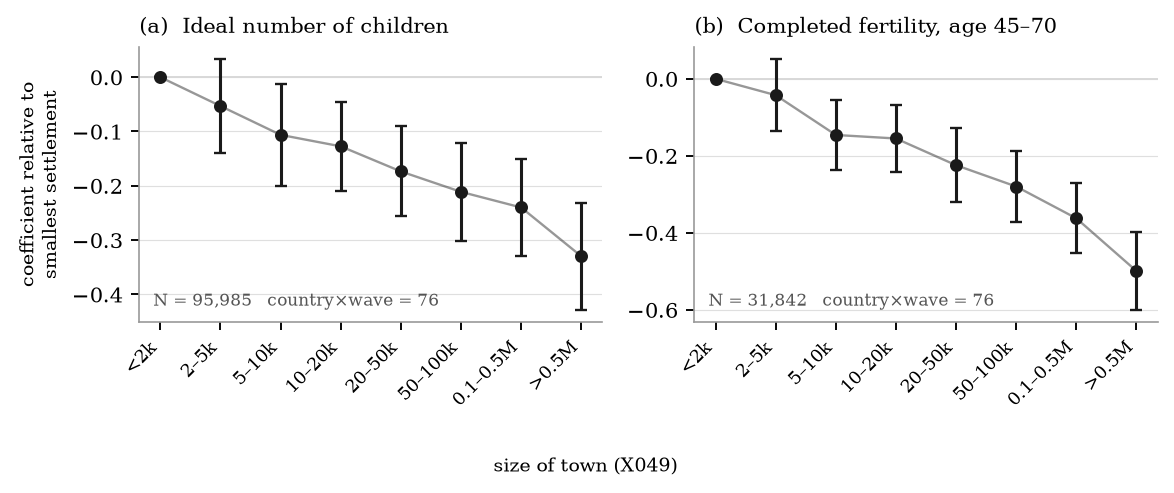
\includegraphics[width=\textwidth]{fig_gradient_v5.png}%
}{%
  \fbox{\parbox[c][0.33\textwidth][c]{\textwidth}{\centering\itshape
  [fig\_gradient\_v5.png --- coefficient plot to be inserted]}}%
}
\caption{Fertility by settlement size. Coefficients $\hat\beta_k$ from \eqref{eq:gradient_spec}
with the smallest settlement ($<2{,}000$) as the omitted category and 95\% confidence intervals,
country$\times$wave fixed effects, controlling for age, sex, marital status and religiosity.
Panel (a) is the ideal number of children (\texttt{D017}, WVS waves 2--4); panel (b) is children
ever had (\texttt{X011}, also WVS waves 2--4) for respondents aged 45--70. WVS version 5.0.
Survey-weighted; standard errors clustered
at the country--wave level.}
\label{fig:gradient}
\end{figure}

The gradient is monotone across all eight bins and in both measures. Relative to settlements under
2{,}000 inhabitants, the ideal number of children falls by $0.053$ in the smallest towns and by
$0.330$ (s.e.\ $0.050$) in cities above half a million; completed fertility falls by $0.499$
(s.e.\ $0.051$) over the same range. This is the micro analogue of the comparative static
$\partial n/\partial \epsilon>0$ of Section~\ref{sec:habitat_taste}.

The bad-control prediction of Section~\ref{sub:ltest} is visible in the same estimates. Adding
education and income --- both chosen jointly with fertility given $\alpha$ --- attenuates the
largest coefficient from $-0.330$ to $-0.275$ for ideal fertility and from $-0.499$ to $-0.390$ for
realised fertility, a compression of roughly a fifth in each case. We therefore report the
specification without them as the headline and the attenuation alongside it rather than in its
place.

We stress what none of this establishes. Because every mechanism in Table~\ref{tab:fingerprints} generates the same pattern,
Figure~\ref{fig:gradient} is a motivating fact and not a test. Nor are settlement bins a measure of
$\epsilon_t=E_t/L_t$: they order respondents by the population of their locality, not by habitat per
person, and they do so in the cross-section rather than along the aggregate time path the model
describes. The next two subsections address these two limitations in turn.

%% -------------------------------------------------------------
\subsection{The identifying test: expenditure shares and labour supply}
\label{sub:ltest}
%% -------------------------------------------------------------

Proposition~\ref{prop:identification} turns the question into one of sign and ratio, and tells us
which ratio to use. The primary test pairs fertility with the education spending share, both
regressed on the same habitat measure over a common sample and with an identical right-hand side:
\begin{align}
\ln n_{it} &= \pi_n \ln \epsilon_{it} + \mathbf{x}_{it}'\boldsymbol{\delta}_n+\tau_t+u_{it},
\label{eq:pair_n}\\
\ln\!\left(p_{it}q_{it}n_{it}/W_{it}\right) &= \pi_{Q}\ln \epsilon_{it}
  + \mathbf{x}_{it}'\boldsymbol{\delta}_{Q}+\tau_t+\upsilon_{it}.
\label{eq:pair_q}
\end{align}
The model predicts
\begin{align}
\pi_n>0,
\qquad
\pi_{Q}<0,
\qquad
\widehat\Lambda'=\hat\pi_{Q}/\hat\pi_n\in[-0.160,\,-0.126],
\label{eq:test}
\end{align}
with the confidence interval for $\widehat\Lambda'$ obtained by the delta method or by a cluster
bootstrap. Every cost channel --- the time cost $\phi$ of \citet{DELACROIX2012271} and
\citet{dao25}, a housing or other per-child goods cost $\kappa$, and the price of education goods
--- predicts $\pi_{Q}=0$ and hence $\Lambda'=0$, because by \eqref{eq:invariants} none of them
touches the expenditure shares. The hypotheses are therefore nested and separately testable, and
failing to reject $\pi_{Q}=0$ is informative against our mechanism rather than merely
uninformative. Either of the other two invariants in \eqref{eq:invariants} --- total education time
$sn$, or the consumption share $c/W$ --- may replace the numerator, with the same predicted value.
If the time cost of children also varies with habitat, as in Section~\ref{sec:timecost}, an
estimate between zero and the band in \eqref{eq:test} is not a rejection of either mechanism: by
\eqref{eq:Lambda_share} it measures the share of the fertility gradient that operates through
tastes.

\paragraph{Is the test powered?}
The restriction in \eqref{eq:test} is a ratio of two small numbers, and what governs its precision
is the dispersion of habitat per capita in the sample, not of settlement size. In the General
Social Survey used below the standard deviation of log size of place is $2.18$, which at
$\beta=0.85$ corresponds to a standard deviation of $\ln\epsilon$ of only $0.33$, three-quarters of
it between primary sampling units. We simulate the two-channel model of
Section~\ref{sec:timecost} from its closed forms under exactly that design: six respondents per
cluster, children drawn as Poisson counts, a cluster shock with standard deviation $0.20$ common to
both equations, and a numerator whose idiosyncratic log standard deviation of $0.9$ is calibrated
to the sampling error of weekly hours in the GSS. The null world has the time cost alone,
calibrated to the same fertility gradient as the alternative, so the two are observationally
identical in the fertility equation.

\begin{table}[h!]\centering
\begin{threeparttable}
\caption{Power of the ratio test under a realistic sampling design}
\label{tab:power}
\footnotesize\setlength{\tabcolsep}{3.5pt}
\begin{tabular}{lrccccc}
\toprule
& & \multicolumn{2}{c}{Cost-only null} & \multicolumn{3}{c}{Taste channel active}\\
\cmidrule(lr){3-4}\cmidrule(lr){5-7}
Fertility gradient & $N$ & s.d. & size & true & mean (s.d.) & power\\
\midrule
Calibrated, $S=0.32$; tastes only          & $37{,}800$  & $0.048$ & $0.04$ & $-0.126$ & $-0.127$ $(0.053)$ & $0.82$\\
                                           & $150{,}000$ & $0.025$ & $0.04$ & $-0.126$ & $-0.129$ $(0.024)$ & $1.00$\\
Calibrated; tastes + time cost, $\chi=0.1$ & $37{,}800$ & $0.048$ & $0.04$ & $-0.097$ & $-0.100$ $(0.040)$ & $0.71$\\
                                           & $150{,}000$ & $0.025$ & $0.04$ & $-0.097$ & $-0.097$ $(0.019)$ & $1.00$\\
Observed in GSS, $S=0.16$; tastes only & $37{,}800$ & $0.096$ & $0.06$ & $-0.126$ & $-0.120$ $(0.109)$ & $0.34$\\
                                           & $150{,}000$ & $0.047$ & $0.04$ & $-0.126$ & $-0.131$ $(0.049)$ & $0.86$\\
                                           & $600{,}000$ & $0.023$ & $0.04$ & $-0.126$ & $-0.126$ $(0.026)$ & $1.00$\\
\bottomrule
\end{tabular}
\begin{tablenotes}\footnotesize
\item 200 replications per row. ``Size'' and ``power'' refer to a one-sided test of $\Lambda=0$ at
the five per cent level against the simulated null distribution. $N=37{,}800$ matches the GSS
estimation sample. $S$ is the habitat elasticity of fertility in \eqref{eq:S_def}.
\end{tablenotes}
\end{threeparttable}
\end{table}

The ratio is estimated without bias in every configuration, and with the fertility gradient of the
calibration a sample of GSS size would detect the taste channel four times in five. The gradient
actually observed in the GSS is half as steep, however, and precision deteriorates in proportion:
the standard error of the ratio doubles to about $0.10$ and power falls to roughly one in three. A
decisive test at the observed gradient needs of the order of $150{,}000$ observations, or a sample
with more dispersion in habitat per capita than a single country provides.

\paragraph{Labour supply as a secondary test.}
Replacing the numerator of \eqref{eq:test} by hours worked gives $\widehat\Lambda_\ell$, which is
weaker but far more widely measured. By \eqref{eq:ell_general} it equals $\Lambda'$ when the cost of
children is purely a time cost, and departs from it as the goods share rises: under the taste
channel it takes the value \eqref{eq:Lambda_ell}, while under a pure goods-cost channel it sweeps
$(-0.128,\,0)$. A labour-supply test therefore still rejects the time-cost channel of
\citet{DELACROIX2012271} and \citet{dao25}, for which $\Lambda_\ell=0$ exactly, but cannot on its
own separate a taste shift from a housing-cost shift. We report it because the US General Social
Survey measures hours worked (\texttt{HRS1}) alongside fertility and size of place of residence,
and so permits the secondary test on a long and familiar sample.

\paragraph{Results from the General Social Survey.}
We implement the secondary test on the GSS cumulative file, 1975--2022, for respondents aged
25--54. Habitat is minus the log of size of place (\texttt{SIZE}, in thousands); fertility is
children ever born (\texttt{CHILDS}); labour supply is weekly hours (\texttt{HRS1}) with
non-workers entered at zero, as the model's $\ell$ requires. Both equations are estimated by
Poisson pseudo-maximum likelihood on a common sample, with year effects and controls for age, sex,
marital status, race, region and religious attendance, post-stratification weights, and a
bootstrap over the $6{,}184$ sampling clusters.

\begin{table}[h!]\centering
\begin{threeparttable}
\caption{The labour-supply ratio $\widehat\Lambda_\ell$ in the General Social Survey}
\label{tab:gss}
\footnotesize\setlength{\tabcolsep}{3.5pt}
\begin{tabular}{lrcccc}
\toprule
Sample and specification & $N$ & $\hat\pi_n$ & $\hat\pi_\ell$ & $\widehat\Lambda_\ell$ & 95\% interval\\
\midrule
Headline                              & $37{,}678$ & $0.0243$ $(0.0027)$ & $-0.0011$ $(0.0022)$ & $-0.046$ & $[-0.204,\,0.142]$\\
\quad + education                     & $37{,}614$ & $0.0190$ $(0.0024)$ & $\phantom{-}0.0038$ $(0.0022)$ & $\phantom{-}0.199$ & $[-0.038,\,0.451]$\\
\quad + education and income          & $34{,}923$ & $0.0196$ $(0.0025)$ & $\phantom{-}0.0053$ $(0.0023)$ & $\phantom{-}0.269$ & $[\phantom{-}0.060,\,0.531]$\\
Women                                 & $20{,}806$ & $0.0204$ $(0.0039)$ & $-0.0064$ $(0.0038)$ & $-0.311$ & $[-0.652,\,0.070]$\\
Men                                   & $16{,}872$ & $0.0300$ $(0.0041)$ & $\phantom{-}0.0028$ $(0.0026)$ & $\phantom{-}0.092$ & $[-0.064,\,0.261]$\\
Married, household hours              & $20{,}916$ & $0.0189$ $(0.0026)$ & $\phantom{-}0.0023$ $(0.0018)$ & $\phantom{-}0.120$ & $[-0.080,\,0.323]$\\
Workers only                          & $28{,}289$ & $0.0285$ $(0.0030)$ & $\phantom{-}0.0003$ $(0.0011)$ & $\phantom{-}0.011$ & $[-0.070,\,0.083]$\\
1975--1998                            & $19{,}389$ & $0.0262$ $(0.0033)$ & $-0.0036$ $(0.0028)$ & $-0.136$ & $[-0.331,\,0.068]$\\
2000--2022                            & $18{,}289$ & $0.0205$ $(0.0043)$ & $\phantom{-}0.0016$ $(0.0032)$ & $\phantom{-}0.078$ & $[-0.211,\,0.418]$\\
\bottomrule
\end{tabular}
\begin{tablenotes}\footnotesize
\item Coefficients are elasticities with respect to minus log size of place; multiply by
$1/(1-\beta)$ to express them per unit of $\ln\epsilon$. Bootstrap standard errors in parentheses
and percentile intervals, 200 replications over sampling clusters. The taste channel alone predicts
$\Lambda_\ell\in[-0.160,-0.126]$; a pure time cost predicts $0$.
\end{tablenotes}
\end{threeparttable}
\end{table}

Two findings emerge, and they pull in different directions. The fertility gradient replicates in
an independent survey of a single country: $\hat\pi_n$ is positive and precisely estimated in every
row, and at $\beta=0.85$ the headline implies a feedback strength of $\hat S=0.162$
$[0.127,\,0.197]$, somewhat below the $0.209$ obtained from the World Values Survey but of the same
order. Labour supply, by contrast, shows no detectable response to habitat. The headline ratio is
$-0.046$ with an interval that contains both zero and the whole of the taste-only band, so the test
discriminates between neither hypothesis --- as Table~\ref{tab:power} leads one to expect at this
sample size. The sign is as the taste channel predicts for women and in the first half of the
sample, where the ratios of $-0.31$ and $-0.14$ are close to or beyond the band, and it is reversed
for men and after 2000. On the intensive margin the evidence is sharper and unfavourable: among
those in work the ratio is $0.011$ with an interval of $[-0.070,\,0.083]$ that excludes the band,
so any response of labour supply to habitat operates through participation and not through hours.
Adding education and income raises the ratio instead of attenuating it; with a headline
indistinguishable from zero that movement cannot be read as the bad-control bias described below.
We also note that the ideal number of children (\texttt{CHLDIDEL}) shows no gradient in size of
place in the GSS, with an elasticity of $0.0018$ (s.e.\ $0.0015$), in contrast to the World Values
Survey.

We conclude that the labour-supply test is not informative at the scale of the GSS. It does not
reject the time-cost channel, and it does not reject the taste channel.

\paragraph{Results from the Consumer Expenditure Survey.}
The primary test requires expenditure, and we take it to the Interview Survey of the US Consumer
Expenditure Survey, 2000--2026: $662{,}987$ quarterly interviews, which we average within consumer
unit to obtain $236{,}529$ households. The estimation sample is the $64{,}853$ units with a
reference person aged 25--44, one or two adults, and positive earnings. Three features of the
implementation matter. First, Proposition~\ref{prop:identification} defines the shares relative to
\emph{full} income $W$, not to spending: relative to consumption, education outlays are the
constant $\gamma\theta$ whatever the habitat. We therefore scale each numerator by the household's
hourly wage, family wage and salary income divided by the annual hours of the reference person and
spouse. Second, the public files report location only as the population class of the sampling
area, five bands plus a rural indicator; habitat is minus the log of the class midpoint, and
inference is by bootstrap over 139 state-by-class cells because sampling-unit identifiers are
withheld for most households. Third, fertility is measured by children under 18 present in the
household. All equations include year effects and controls for age, sex, marital status, race and
region, and are weighted.

\begin{table}[h!]\centering
\begin{threeparttable}
\caption{Expenditure-share and labour-supply ratios in the Consumer Expenditure Survey}
\label{tab:cex}
\footnotesize\setlength{\tabcolsep}{4pt}
\begin{tabular}{lccc}
\toprule
Outcome & Habitat elasticity & Ratio to $\hat\pi_n$ & 95\% interval\\
\midrule
\multicolumn{4}{l}{\emph{A. Headline: earners, $N=64{,}853$}}\\
Children under 18, $\hat\pi_n$                    & $\phantom{-}0.0370$ $(0.0053)$ & & \\
Education spending / wage                         & $-0.0129$ $(0.0166)$ & $-0.35$ & $[-1.29,\,0.43]$\\
Any education spending                            & $\phantom{-}0.0036$ $(0.0052)$ & $\phantom{-}0.10$ & $[-0.21,\,0.34]$\\
Consumption / wage                                & $\phantom{-}0.0088$ $(0.0024)$ & $\phantom{-}0.24$ & $[\phantom{-}0.13,\,0.34]$\\
Household annual hours                            & $-0.0123$ $(0.0021)$ & $-0.33$ & $[-0.45,\,-0.24]$\\
Hourly wage                                       & $-0.0586$ $(0.0060)$ & & \\
\midrule
\multicolumn{4}{l}{\emph{B. Conditioning on the log wage}}\\
Children under 18, $\hat\pi_n$                    & $\phantom{-}0.0326$ $(0.0054)$ & & \\
Education spending / wage                         & $-0.0259$ $(0.0160)$ & $-0.80$ & $[-1.94,\,0.07]$\\
Consumption / wage                                & $-0.0229$ $(0.0032)$ & $-0.70$ & $[-1.08,\,-0.53]$\\
Household annual hours                            & $-0.0129$ $(0.0023)$ & $-0.39$ & $[-0.55,\,-0.28]$\\
\midrule
\multicolumn{4}{l}{\emph{C. All one- and two-adult households, $N=74{,}902$}}\\
Children under 18, $\hat\pi_n$                    & $\phantom{-}0.0353$ $(0.0049)$ & & \\
Household annual hours, non-workers at zero       & $-0.0103$ $(0.0018)$ & $-0.29$ & $[-0.44,\,-0.20]$\\
\bottomrule
\end{tabular}
\begin{tablenotes}\footnotesize
\item Elasticities with respect to minus the log population of the sampling area. Education
spending is winsorised at the 99th percentile and estimated by Poisson pseudo-maximum likelihood,
as are the counts and the hours in panel C; consumption, hours in panels A and B, and the wage are
in logs. Consumption is total expenditure less education. Bootstrap standard errors in
parentheses and percentile intervals, 200 replications. Tastes alone predict a ratio in
$[-0.160,-0.126]$ for the shares; any cost channel predicts $0$.
\end{tablenotes}
\end{threeparttable}
\end{table}

The fertility gradient appears for a third time, in a third survey: $\hat\pi_n=0.037$, or
$\hat S=0.25$ $[0.18,\,0.32]$ at $\beta=0.85$, close to the World Values Survey estimate. Beyond
that the results are sobering for the identification strategy, and we report them as they are.

The education share, the numerator on which Section~\ref{sub:restrictions} places most weight, is
uninformative. Fewer than a third of these households report any education outlay while in the survey, the
amounts are highly skewed and include adults' own tuition, and the ratio of $-0.35$ carries an
interval, $[-1.29,\,0.43]$, that contains zero, the taste band and a great deal else.

The consumption share is precisely estimated but does not behave as either hypothesis requires.
Unconditionally it \emph{rises} with habitat, giving a ratio of $0.24$ that rejects both the
taste band and zero. Conditional on the wage it falls, with a ratio of $-0.70$ that has the sign of
the taste channel and several times its magnitude. The reversal identifies the problem. Wages are
six per cent lower per log point of habitat, and consumption relative to the wage declines steeply
in the wage itself, whereas the logarithmic preferences behind
Proposition~\ref{prop:identification} impose a unit income elasticity and hence shares that are
independent of $W$. That invariance fails in the data, and with it the claim that the shares move
with habitat only through $\alpha$: the estimated ratio takes whatever sign the treatment of the
wage gives it.

Labour supply is more robust. Household hours fall with habitat in every specification, with a
ratio between $-0.29$ and $-0.39$ and intervals that exclude zero. This rejects the pure time-cost
channel, for which $\Lambda_\ell=0$, and it has the sign that both the taste channel and a
goods-cost channel predict; it is also larger than either can deliver, which points to the
violation flagged below, that labour supply responds directly to the lower wages of less dense
areas. It stands in contrast to the GSS, where no response was detectable.

We draw three conclusions. The habitat gradient in fertility is a robust fact across three surveys
and a cross-country panel. The pure time-cost account of that gradient is rejected on the
labour-supply margin in the larger of the two US samples, though not in the smaller. And the
expenditure-share test cannot at present separate tastes from goods costs: its sharp prediction
rests on homothetic preferences that these data reject, so that a credible version requires either
a preference specification with non-unitary income elasticities or variation in habitat that is
orthogonal to local wages.

\paragraph{A by-product: the composition of the cost of children.}
Because $\Lambda'$ is invariant to $\psi$ and $\Lambda_\ell$ is not, estimating both identifies the
time share of the cost of children. The cleanest route is through levels rather than elasticities:
$s_tn_t$ is observable as total time devoted to children's education and is equal to
$\gamma\eta/(1+\alpha_t)$ by \eqref{eq:invariants}, so $\phi n_t=1-\ell_t-s_tn_t$ and
\begin{align}
\psi_t=\frac{\left(1-\ell_t-s_tn_t\right)\left(1+\alpha_t\right)}{\alpha_t-\Gamma},
\label{eq:psi_identified}
\end{align}
with $\alpha_t$ recovered from any of the invariants. The share of the cost of children borne as
time rather than goods is a quantity the density literature argues over and has not pinned down;
our framework delivers it as a by-product of the identification exercise rather than as a separate
undertaking.

\paragraph{Qualifications.}
Two apply to both tests. The model has homogeneous adults, whereas in the data the labour-supply
margin is overwhelmingly female; we therefore estimate the secondary test separately by sex and
treat the household-level prediction as the one the theory speaks to. And the ratios are joint
tests of the mechanism and of the exclusion restriction that settlement size affects the numerator
only through the fertility taste. We report the sensitivity of both estimates to local wage and
industry-composition controls, which is the most plausible violation. A third qualification is
specific to the model: $s$, $q$ and labour income are chosen jointly with $n$ and $\ell$ given
$\alpha$, so conditioning on education or on labour income conditions on an outcome of the
mechanism and biases both ratios toward zero. The headline specifications omit both, and we report
the attenuation as controls are added rather than suppressing it.


%% -------------------------------------------------------------
\subsection{Estimating $\xi$ by inverting the fertility rule}
\label{sub:xi}
%% -------------------------------------------------------------

The calibration of Section~\ref{sec:calibration} set the elasticity $\xi$ in
$\alpha(\epsilon)=\alpha_0\epsilon^{\xi}$ by an illustrative target: the value at which a doubling of
habitat per capita brings fertility to replacement, giving $\xi=0.146$. The data allow $\xi$ to be
estimated rather than imposed. The key observation is that the fertility rule
\eqref{eq:sol_n_hab} inverts in closed form.

\begin{proposition}[Recovering the fertility taste from observed fertility]
\label{prop:inversion}
For any $n<1/\phi$, the fertility rule $n=(\alpha-\Gamma)/[\phi(1+\alpha)]$ inverts to
\begin{align}
\alpha=\mathcal{A}(n)\equiv\frac{\phi n+\Gamma}{1-\phi n},
\qquad
\mathcal{A}'(n)=\frac{\phi(1+\Gamma)}{(1-\phi n)^{2}}>0 .
\label{eq:inversion}
\end{align}
At $n=1$, $\mathcal{A}(1)=(\phi+\Gamma)/(1-\phi)=\alpha^{\ast}$, the replacement-fertility taste of
Remark~\ref{rem:eps_stability_hab}.
\end{proposition}

Given $(\phi,\Gamma)$ from the calibration, \eqref{eq:inversion} maps any observed fertility rate
into the taste parameter that rationalises it. Applying it cell by cell --- we use country
$\times$ wave $\times$ settlement-bin cells, so that $n$ is a cell mean rather than an individual
count --- yields $\hat\alpha_{j}$ for each cell $j$. The elasticity is then the slope of
\begin{align}
\ln \hat\alpha_{j}=\ln\alpha_0+\xi \ln \epsilon_{j}+\mu_{c}+\tau_{w}+\zeta_{j}.
\label{eq:xi_spec}
\end{align}

We implement \eqref{eq:xi_spec} on country$\times$wave$\times$bin cells built from \texttt{X011}
for respondents aged 45--70, taking $n$ as half the cell's weighted mean number of children so that
$n=1$ is replacement, and keeping cells with at least thirty respondents. This yields $1{,}034$
cells across $226$ country--waves. The unweighted mean implied taste across cells is $\hat\alpha=0.503$, above both
$\alpha_0$ and $\alpha^{\ast}$, as one expects in a global sample whose older cohorts completed
their fertility above replacement.

Implementing \eqref{eq:xi_spec} requires $\epsilon$ in levels, which the settlement bins do not
provide: they record the \emph{population} of a locality, not space per person. Writing
$\beta$ for the elasticity of a locality's land area with respect to its population, density scales
as population to the power $1-\beta$, and the regression of $\ln\hat\alpha_j$ on minus the log of
bin-midpoint population identifies $\xi(1-\beta)$ rather than $\xi$ itself. That composite is
estimated precisely,
\begin{align}
\widehat{\xi(1-\beta)}=0.0185\quad(\text{s.e.}\ 0.0012),
\label{eq:xi_composite}
\end{align}
and is stable across the choices the construction forces on us: it lies between $0.017$ and $0.022$
when the open top bin is assigned a midpoint of $0.75$, $1$ or $2$ million, when the minimum cell
size is $15$ or $50$, when the age window is $40$--$75$ or $50$--$70$, when the sample is restricted
to women, and when it is split into waves 2--4 and waves 5--7. The $\hat\alpha_j$ are also monotone
in bin, falling by $0.129$ log points from the smallest settlements to cities above half a million.

Recovering $\xi$ itself requires a value for $\beta$. Land area scales sublinearly with population,
and at the value of $\beta=0.85$ commonly used in the urban-scaling literature
\eqref{eq:xi_composite} implies
\begin{align}
\hat\xi=0.123\qquad[0.108,\,0.139],
\label{eq:xi_estimate}
\end{align}
against the $0.146$ imposed in Section~\ref{sec:calibration}; the calibrated value is reproduced
exactly at $\beta=0.873$. Two qualifications govern how this number should be read. The inference from
\eqref{eq:xi_composite} to \eqref{eq:xi_estimate} rests on $\beta$ and not on anything the survey
measures. And by \eqref{eq:xi_bound} the inversion attributes the whole fertility gradient to
tastes, so that \eqref{eq:xi_estimate} estimates $\xi+\chi/\mathcal{K}$: the total habitat
elasticity of fertility in taste units, and an upper bound on $\xi$ itself. A time-cost elasticity
of $\chi=0.1$ would lower the implied taste elasticity to $0.070$. Separating the two requires the
expenditure-share regression of Section~\ref{sub:ltest} and the decomposition
\eqref{eq:decomposition}. What the data establish without taking a view on the mix is the feedback strength $S$ of
Proposition~\ref{prop:two_channels}, which is simply the habitat elasticity of fertility.
Regressing $\ln n_j$ directly on the same regressor gives $\widehat{S(1-\beta)}=0.0313$
(s.e.\ $0.0020$), hence at $\beta=0.85$
\begin{align}
\hat S=0.209\qquad[0.182,\,0.236],
\label{eq:S_estimate}
\end{align}
which implies monotone convergence with a half-life of about three generations. The estimate moves
to $0.16$ at $\beta=0.80$ and $0.31$ at $\beta=0.90$, remaining far from the oscillation threshold
throughout. Read through \eqref{eq:S_def} at the sample mean of $\hat\alpha$, where
$\mathcal{K}=1.57$, it bounds the taste elasticity at $0.133$ if $\chi=0$, and implies $0.069$ at
$\chi=0.1$ and zero at $\chi=0.21$.

\paragraph{A cross-country panel.}
The UN World Population Prospects 2024 provide a check that needs no assumption about $\beta$,
because national population density is observed directly. For 161 countries with at least one
million inhabitants over 1950--2023 we apply the inversion to $n=\text{TFR}/2.1$ and regress
$\ln\hat\alpha$ on $\ln(1/\text{density})$. The slope is $0.059$ (s.e.\ $0.017$) in the 2023
cross-section and $0.103$ (s.e.\ $0.019$) in the pooled sample with year effects; with country and
year effects it is $0.243$ (s.e.\ $0.035$), rising to $0.381$ (s.e.\ $0.032$) after 1990. Every
estimate has the predicted sign. The between-country estimates lie below the survey-based
$0.123$ and the within-country estimates above it, as one would expect: the former are attenuated
by the crudeness of national density as a measure of habitat, while the latter load the
demographic transition, during which density rose and fertility fell for reasons held fixed in the
model, onto the habitat elasticity. We regard the survey estimate, bracketed by the two, as the
more credible.

Had $\hat\xi$ come out substantially smaller, the consequence would have been more than
quantitative: by Remark~\ref{rem:eps_stability_hab}, local stability of $\epsilon^{\ast}$ requires
$0<\epsilon^{\ast}n'(\epsilon^{\ast})<2$, and a weak habitat response places the economy near the
lower edge of that corridor, so that the self-correcting demography on which our main result depends
would operate only slowly. At $\hat\xi\approx0.12$ the estimated total response sits close to the value assumed throughout,
comfortably inside the corridor and well short of the oscillation threshold $S=1$ of
Proposition~\ref{prop:two_channels}, whichever channel accounts for it.

%% -------------------------------------------------------------
\subsection{A cross-country consistency check}
\label{sub:crosscountry}
%% -------------------------------------------------------------

Before turning to what the exercises above cannot settle, we report a check that can be carried out
immediately, because it requires no micro data at all. Proposition~\ref{prop:inversion} maps an
observed fertility rate into the taste parameter that rationalises it, and
$\alpha(\epsilon)=\alpha_0\epsilon^{\xi}$ then maps that taste into the habitat per capita the model
requires. Running both steps on observed national fertility therefore produces, for each country, a
\emph{predicted population density} --- a quantity the model has no business getting right, and one
that can be compared with the observed figure.

The exercise has exactly one free normalisation, which we state explicitly. The model's own baseline
is $\epsilon=1$, at which $\alpha=\alpha_0=0.39$ and hence $n=0.813$: with replacement at a total
fertility rate of $2.1$, that corresponds to a TFR of $1.71$. We anchor $\epsilon=1$ to
$D_0=120.5$ inhabitants per square kilometre, the density of France, whose TFR of $1.64$ is the
closest in our sample to the model's baseline. Nothing else is chosen: $\xi=0.146$, $\phi$ and
$\Gamma$ are all carried over unchanged from Section~\ref{sec:calibration}, and every other entry in
Table~\ref{tab:crosscountry} follows mechanically.

\begin{table}[h!]\centering
\begin{threeparttable}
\caption{Model-implied and observed population density, 2023}
\label{tab:crosscountry}
\begin{tabular}{lcccrrcc}
\toprule
& & & & & & \multicolumn{2}{c}{observed / implied}\\
\cmidrule(lr){7-8}
& TFR & $\hat\alpha$ & $\hat\epsilon$ & $D_0/\hat\epsilon$ & observed $D$ & $\xi=0.146$ & $\xi=0.123$\\
\midrule
Korea       & $0.72$ & $0.295$ & $0.149$ & $810$ & $523$  & $0.65$ & $0.45$\\
Taiwan      & $0.87$ & $0.309$ & $0.202$ & $596$ & $658$  & $1.11$ & $0.82$\\
Japan       & $1.21$ & $0.340$ & $0.394$ & $306$ & $330$  & $1.08$ & $0.91$\\
Italy       & $1.20$ & $0.339$ & $0.386$ & $312$ & $201$  & $0.64$ & $0.54$\\
France      & $1.64$ & $0.383$ & $0.883$ & $137$ & $120$  & $0.88$ & $0.86$\\
Singapore   & $0.94$ & $0.316$ & $0.234$ & $514$ & $8{,}476$ & $16.48$ & $12.56$\\
\bottomrule
\end{tabular}
\begin{tablenotes}\footnotesize
\item Total fertility and population density (inhabitants per square kilometre) are 2023 estimates
from UN World Population Prospects 2024. $\hat\alpha=\mathcal{A}(\text{TFR}/2.1)$ from
\eqref{eq:inversion}; $\hat\epsilon=(\hat\alpha/\alpha_0)^{1/\xi}$, shown for the calibrated
$\xi=0.146$. France anchors $\epsilon=1$ at $D_0=120.5$. The last column repeats the comparison at
the survey estimate \eqref{eq:xi_estimate}.
\end{tablenotes}
\end{threeparttable}
\end{table}

The ordering is correct throughout and the magnitudes are close. Taiwan and Japan are matched to
within about ten per cent and France to within twelve; Korea and Italy are the two cases where the
observed density falls short of what the model requires, meaning that their fertility is lower than
the habitat channel alone accounts for. At the smaller survey estimate $\xi=0.123$ the model needs
more crowding to rationalise a given fertility shortfall, and every ratio falls: Taiwan, Japan and
France remain within twenty per cent, while Korea and Italy move to roughly half. For a one-parameter preference shifter whose elasticity was
fixed in Section~\ref{sec:calibration} for an unrelated reason, agreement of this order across a
twentyfold range of densities is more than the exercise was entitled to expect.

Two cautions keep us from claiming more. Singapore is off by a factor of sixteen, as any city-state
must be: crude density is not measuring habitat where there is no hinterland. And the result is
sensitive to the land concept. Crude density happens to fit well, but replacing it with habitable
land --- arguably the better proxy for $E_t$ --- would raise the mountainous cases of Korea and Japan
several-fold and turn their close agreement into substantial overshooting. That sensitivity is a
reason to read Table~\ref{tab:crosscountry} as a consistency check rather than as evidence.

\paragraph{The residual: levels, not changes.}
The check above is cross-sectional. Its time-series counterpart does not pass. Korea's
population rose from 26 to 52 million between 1960 and 2023, halving habitat per capita; at
$\xi=0.146$ this moves the model's fertility from a TFR of $1.71$ to $1.34$, whereas Korean
fertility fell from $6.0$ to
$0.72$. The habitat channel can therefore account for why Korea sits far below other high-income
countries at a point in time, but for only a modest part of its decline over time. This is not a
refutation --- the model never claimed to explain the demographic transition, most of which operates
through forces held fixed here --- but it does mean the channel is partial. It also leaves the
central dynamic prediction untested: stabilisation at $\epsilon^{\ast}$ requires population decline
to raise $\epsilon$, and in no country has that yet begun on a scale that would show up in fertility.
The cross-section can show that the mechanism is present; only time can show that it stabilises.

%% -------------------------------------------------------------
\subsection{What these exercises cannot settle}
\label{sub:caveats}
%% -------------------------------------------------------------

Two limitations deserve to be stated plainly rather than managed.

First, the relationship is simultaneous by construction. This section attempts to
measure $\alpha(\epsilon)$, but the model of Section~4 makes $\alpha_t$ the solution to a
within-period fixed point in which habitat depends on output and output depends on labour supply,
which depends on $\alpha_t$. The empirical counterpart of that simultaneity is residential sorting:
households that want children move to roomier places. Our estimates are therefore associations
consistent with the mechanism, not causal estimates of it, and we do not claim otherwise.

Second, $\epsilon$ in the model is an economy-wide aggregate, while settlement size is local.
Reading the cross-sectional gradient as evidence on $\alpha(\cdot)$ requires assuming that the same
preference function maps local and national roominess into the taste for children. This is an
assumption about the object being measured, not about measurement error, and it is not testable
within these data.

\singlespacing
 \bibliographystyle{chicago}
 	\bibliography{resources}
\end{document}
